\documentclass[10pt,aspectratio=169,dvipsnames]{beamer}
\usetheme[]{Berlin}

\setbeamertemplate{footline}{
  \usebeamercolor[fg]{framesource}%
  \usebeamerfont{page number in head}%
  \hspace{0.2cm}
  \small \insertframenumber
  \vspace{0.2cm}
  \doclicenseIcon
  \hfill
  
\includegraphics[height=0.8cm]{logos/tub_logo.pdf}
  \hspace{0.2cm}
}

\setbeamercovered{transparent}

\setbeamertemplate{footline}[
 myframe number]

% PACKAGES
\usepackage[absolute,overlay]{textpos}
\usepackage[utf8]{inputenc}
\usepackage[official]{eurosym}
\usepackage{booktabs,multicol,multirow,tabularx,array}
\usepackage{subcaption}
\usepackage{parskip}
\usepackage{bm}
\usepackage{tikz}
\usepackage{adjustbox}
\usepackage[super]{nth}
\usepackage[version=4]{mhchem}
\usepackage{siunitx}
\sisetup{
  detect-all = true
}


\usepackage[
    type={CC},
    modifier={by},
    version={4.0},
]{doclicense}

% HYPERREFERENCES
\usepackage{hyperref}
\hypersetup{
	colorlinks=true,
	citecolor=tub-blue,
	linkcolor=tub-blue,
	urlcolor=tub-blue
}

\usepackage[sfdefault]{roboto}
\usepackage[normalem]{ulem}

\usepackage[backend=biber,style=numeric-comp]{biblatex}
\addbibresource{references.bib}

\newcolumntype{R}[1]{>{\raggedleft\arraybackslash}p{#1}}


% GRAPHICS	
\graphicspath{
    {graphics/},
    {../../paper/first-draft/figures} % study results
  }
\DeclareGraphicsExtensions{.pdf,.jpeg,.png,.jpg}

% FORMATTING
\setlength{\parskip}{6pt}
\linespread{1.1}
\newcommand{\seprule}{\par\noindent\textcolor{black!25}{\rule{\textwidth}{0.4pt}}}

% SOURCES
\setbeamercolor{framesource}{fg=gray}
\setbeamerfont{framesource}{size=\tiny}
\newcommand{\source}[1]{\begin{textblock*}{10cm}(3.6cm,8.25cm)
    \begin{beamercolorbox}[ht=0.5cm,right]{framesource}
        \usebeamerfont{framesource}\usebeamercolor[fg]{framesource} Source: {#1}
    \end{beamercolorbox}
\end{textblock*}}

% REFERENCES
% \usepackage[style=nature, doi=true, maxcitenames=3]{biblatex}
% \bibliography{bibliography}
% \renewcommand*{\bibfont}{\footnotesize}

% COLOR TEXT
\newcommand{\bl}[1]{\textcolor{tub-blue}{#1}}
\newcommand{\gr}[1]{\textcolor{tub-green}{#1}}
\newcommand{\rd}[1]{\textcolor{tub-red}{#1}}
\newcommand{\yl}[1]{\textcolor{tub-yellow}{#1}}
% \newcommand{\org}[1]{\textcolor{tub-orange}{#1}}
\newcommand{\cb}[1]{\colorbox{gray!20}{#1}}

\usepackage{array}% https://ctan.org/pkg/array
\makeatletter
\g@addto@macro{\endtabular}{\rowfont{}}% Clear row font
\makeatother
\newcommand{\rowfonttype}{}% Current row font
\newcommand{\rowfont}[1]{% Set current row font
   \gdef\rowfonttype{#1}#1%
}
\newcolumntype{L}{>{\rowfonttype}l}

% Custom commands
\usepackage{caption}
\renewcommand{\figurename}{} % Removes the "Figure" text
\captionsetup[figure]{labelformat=empty, labelsep=none} % Removes numbering and colon


% FONT
%\usepackage{utopia}

% REFERENCES
%\usepackage[backend=biber,style=authoryear-comp]{biblatex}
%\bibliography{references.bib}

% TITLE PAGE
\title{
  \textbf{RESILIENT}\\\nth{2} consortium meeting
}
\vspace*{-.5cm}

% \author{STRIse}
\institute[Technische Universität Berlin] % (optional, but mostly needed)
{ 
  \normalsize
  \alert{The Role of Projects of Common Interest in Reaching Europe's Energy Policy Targets} \\
  \footnotesize
  Bobby Xiong, Iegor Riepin, Tom Brown \\
  \href{mailto:xiong@tu-berlin.de}{xiong@tu-berlin.de} \\
  % Department of Digital Transformation in Energy Systems \\
  Technische Universität Berlin, Germany \\

  \vspace{0.3cm}

  May 15, 2025
}

\date{}

\subject{Recent Research with PyPSA-Eur}

\titlegraphic{%
\vspace{-1cm}

\includegraphics[height=1cm,clip=true]{logos/cetp_logo.png}
\hspace{0.5cm}
\includegraphics[height=1cm,clip=true]{logos/ensys_short_logo.pdf}
\hspace{0.5cm}
\includegraphics[trim=0 0cm 0 0cm,height=1cm,clip=true]{logos/tub_logo.pdf}
\hspace{0.5cm}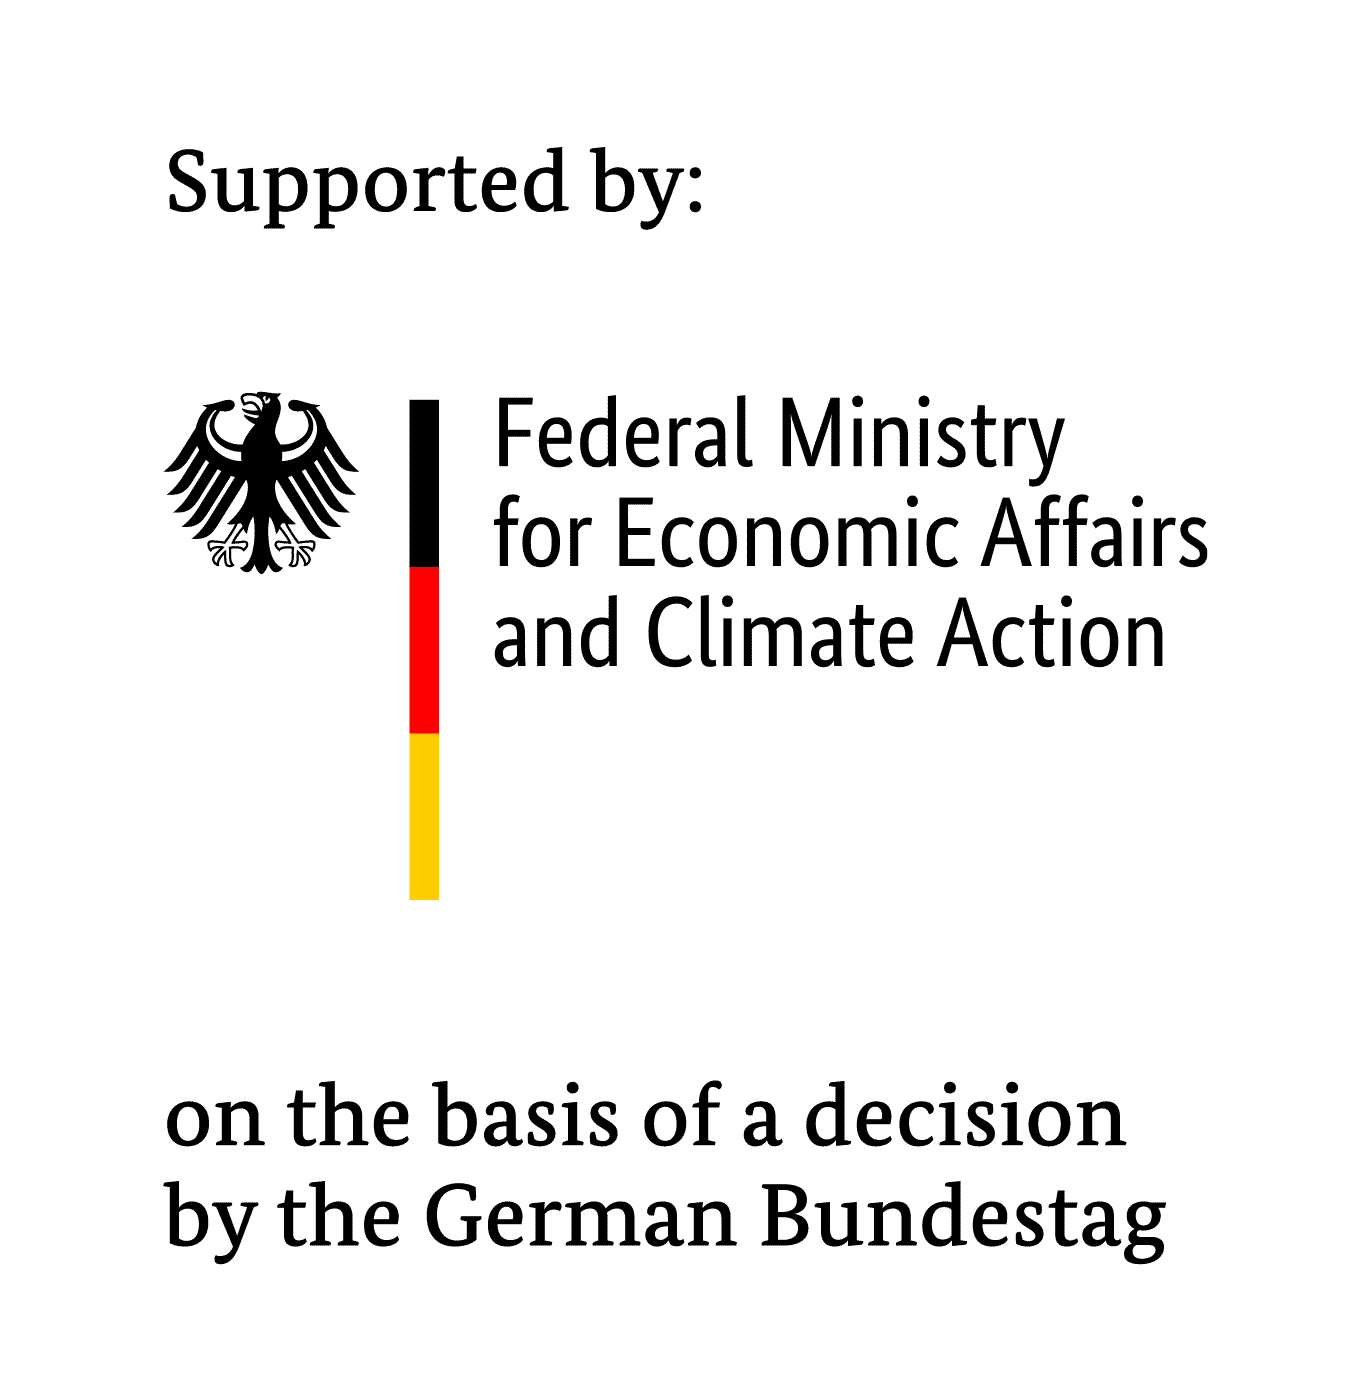
\includegraphics[trim=0.2cm 0.6cm 0.6cm 0.2cm,height=1.1cm,clip=true]{logos/bmwk_en_logo.png}
}


\begin{document}

\addtocounter{framenumber}{-1}
{
  \setbeamertemplate{footline}{
    \usebeamercolor[fg]{framesource}%
    \usebeamerfont{page number in head}%
    \begin{center}
      \Large
      \doclicenseIcon
      \vspace{0.4cm}
    \end{center}
  } 
  \maketitle
}

% \section{Introduction}


% \begin{frame}{RESILIENT project partners}
%   \centering
%   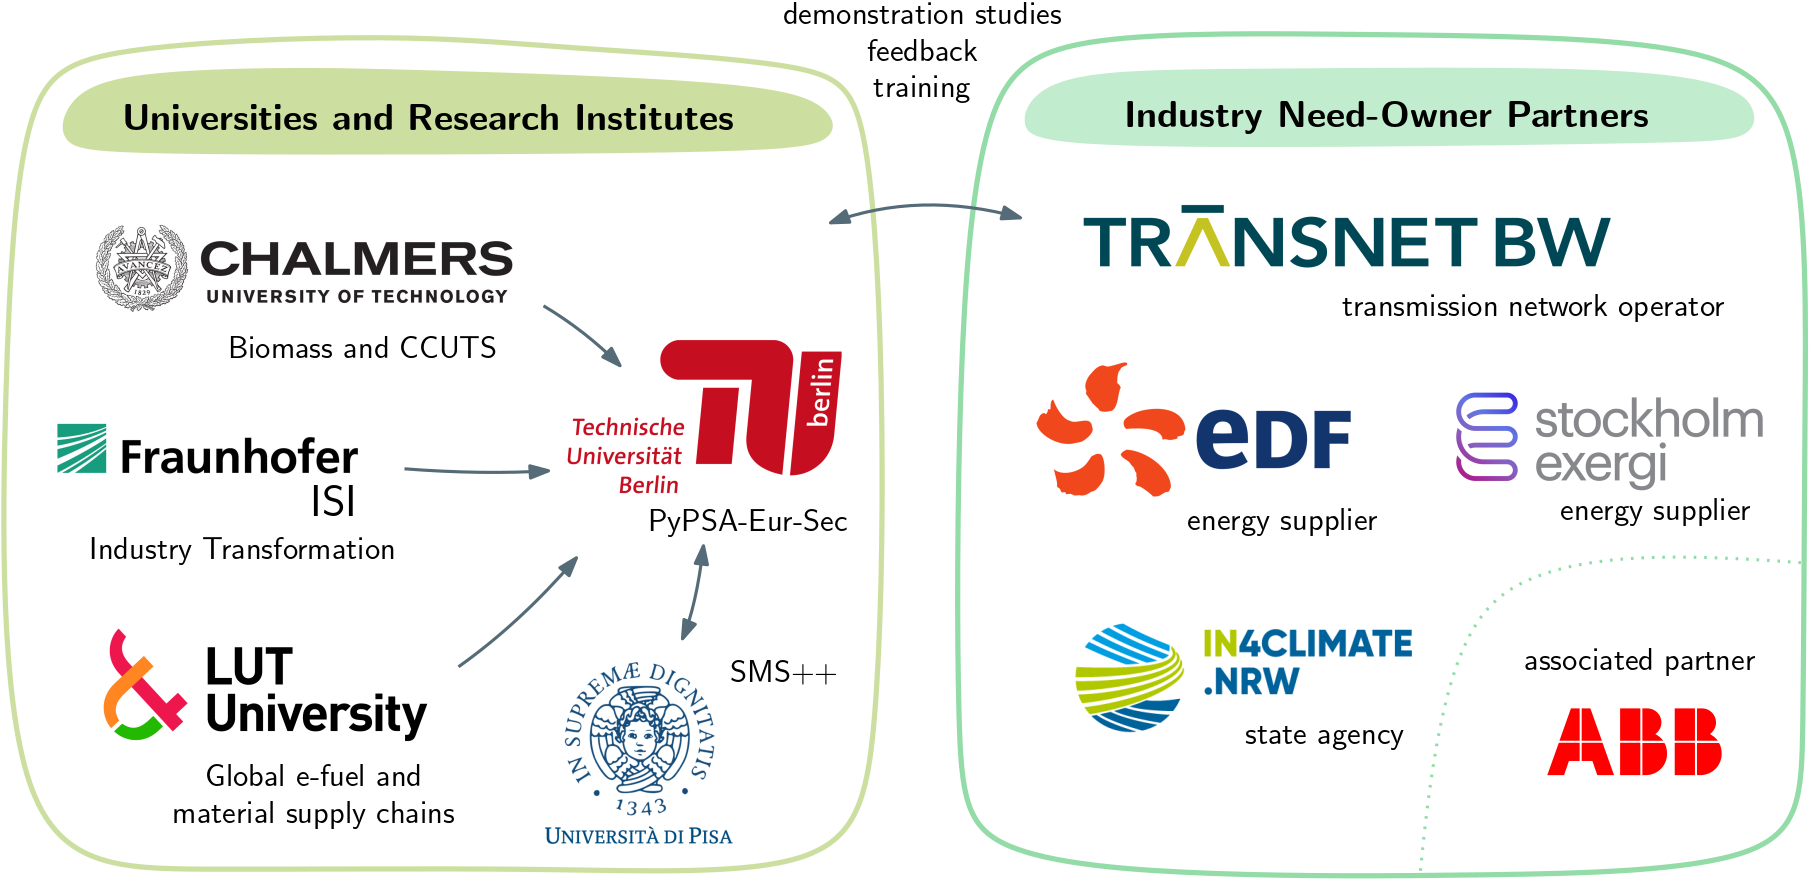
\includegraphics[width=0.85\textwidth]{other/resilient_partners}
  
%   \footnotesize
%   Funded via \alert{CETPartnership 2022} Call --- \alert{BMWK} for all German partners.

%   \source{\url{https://resilient-project.github.io/}}
% \end{frame}

% \begin{frame}{RESILIENT work packages}
%   \centering
%   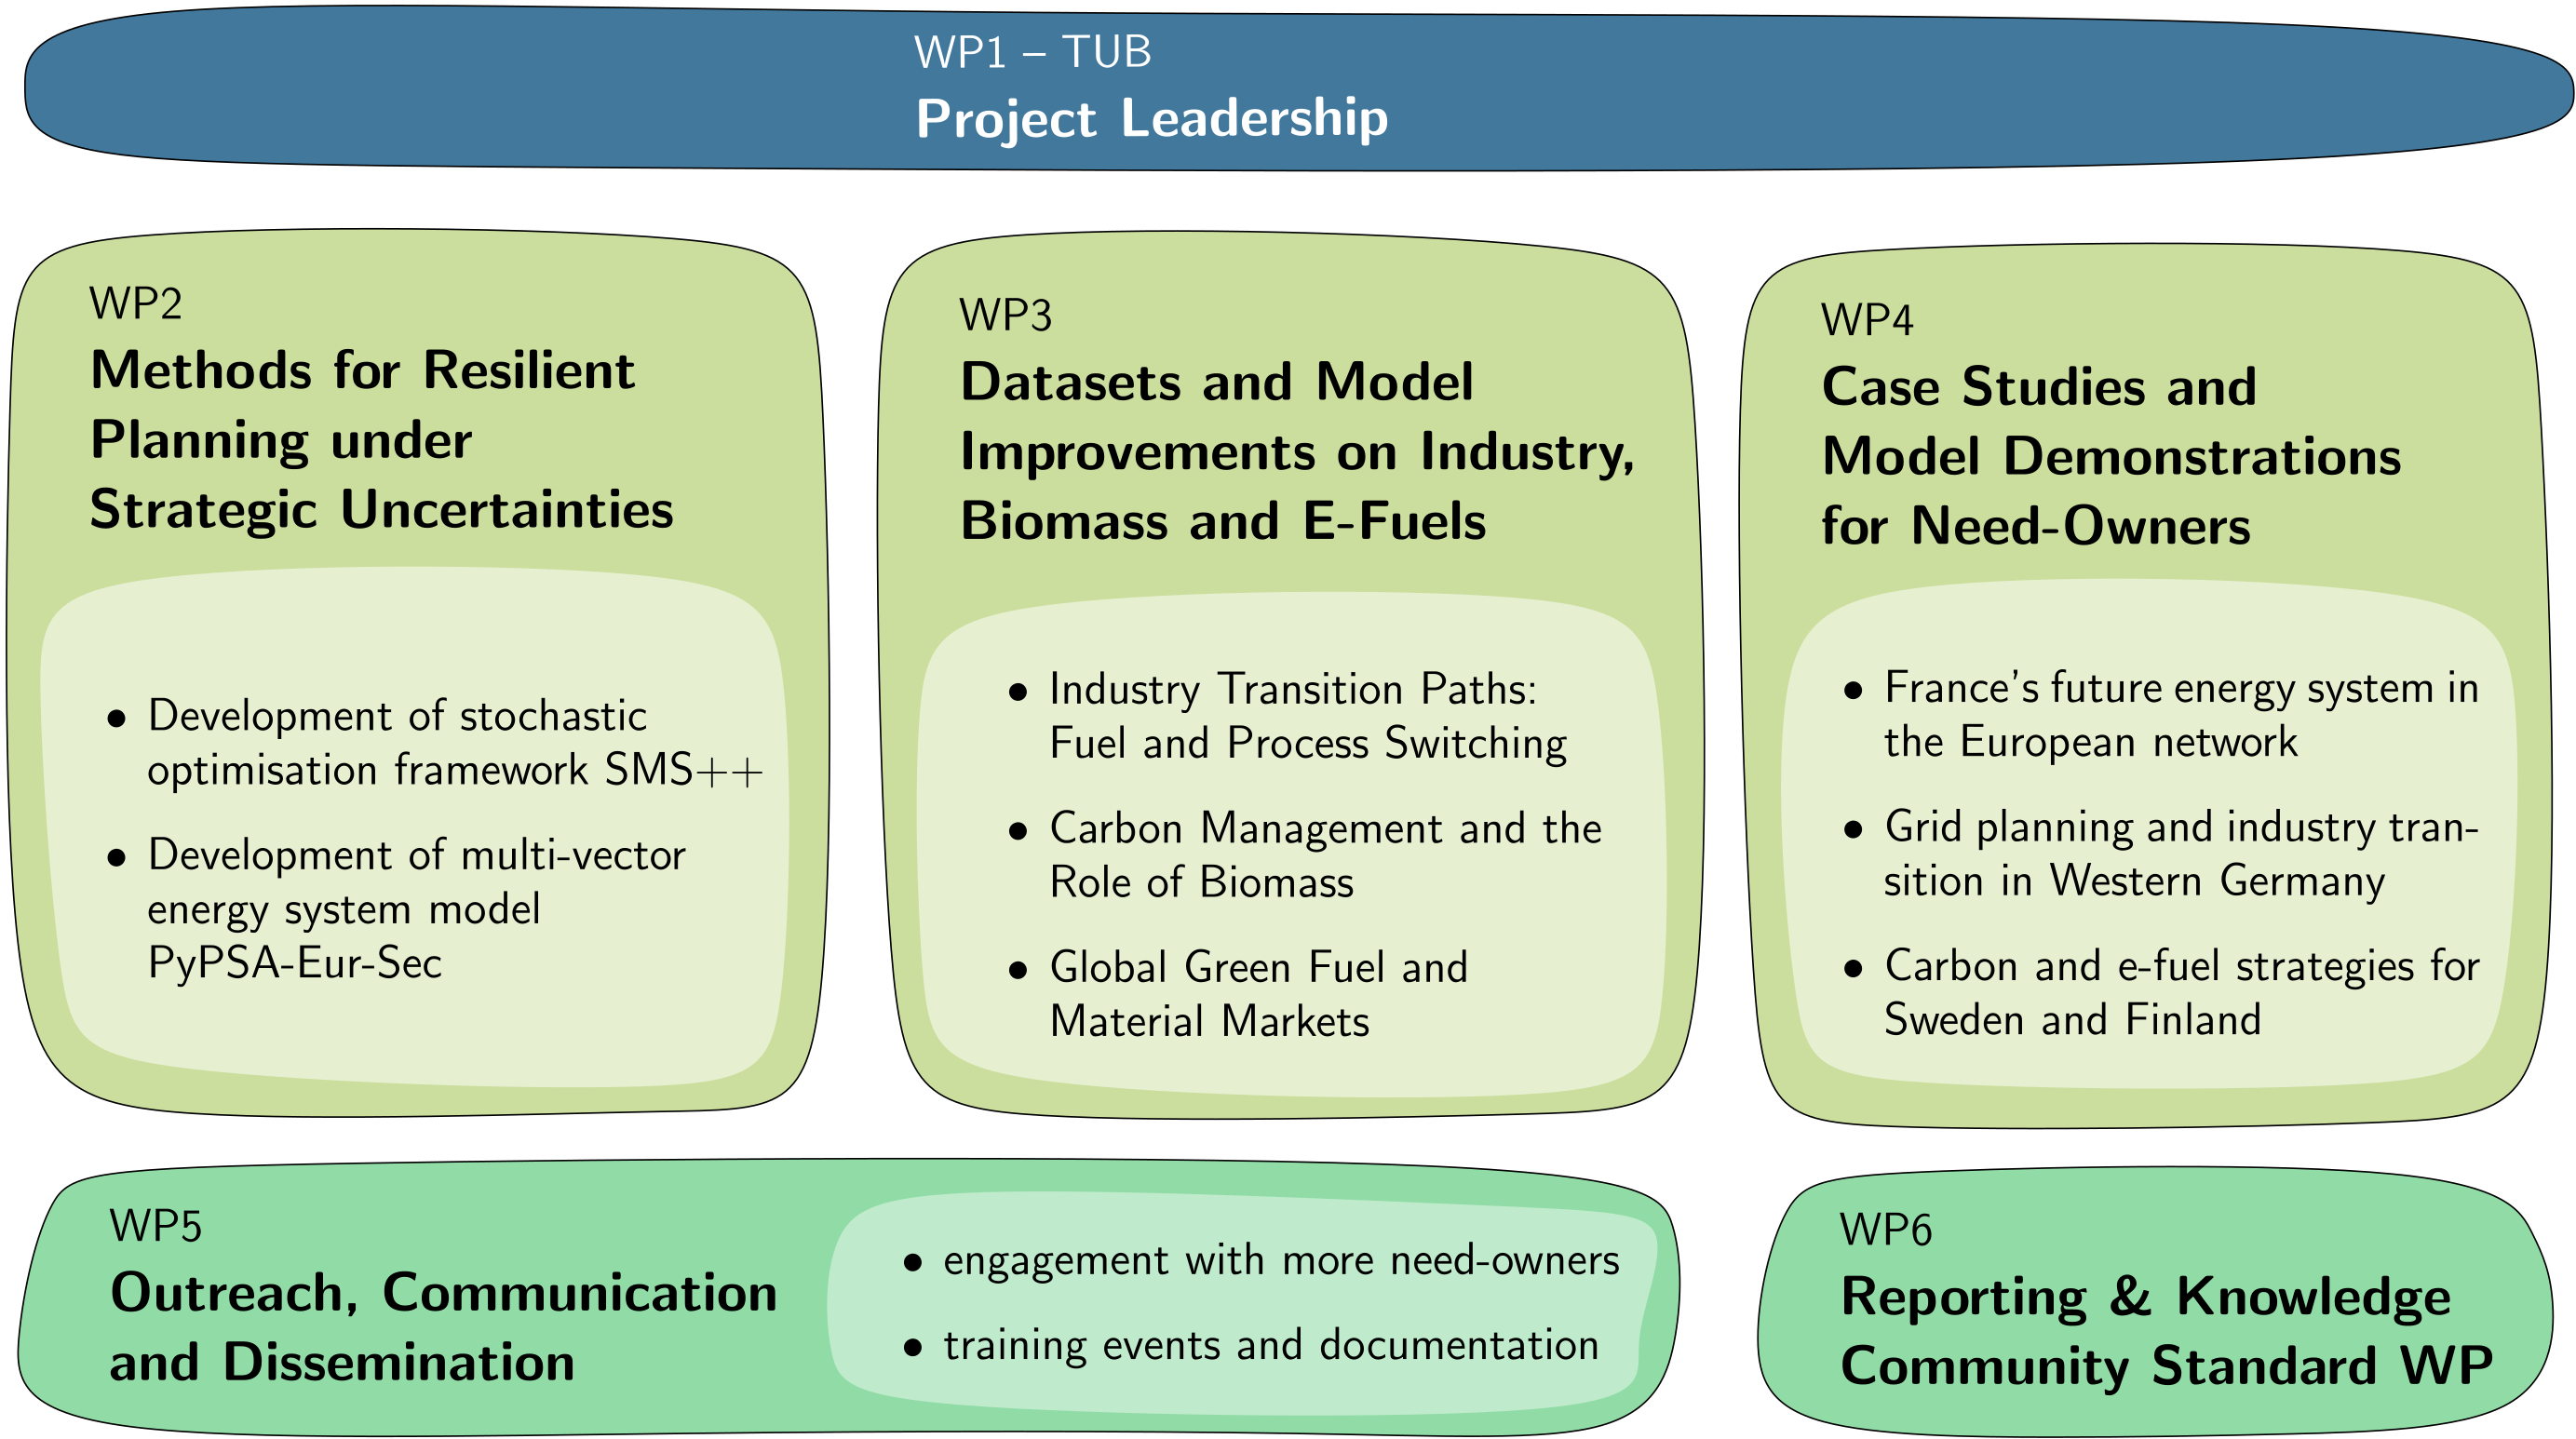
\includegraphics[width=0.8\textwidth]{other/resilient_project_structure}
% \end{frame}

% \begin{frame}{PyPSA-Eur: An open-source, sector-coupled model for Europe}
%   \begin{columns}
%     \begin{column}{0.5\textwidth}
%       \footnotesize
%       \begin{itemize}
%         \setlength\itemsep{.8em}
%         \item Spatially and temporally highly resolved linear optimisation model that covers the \alert{European} continent,
%         \item Built on top of the open-source toolbox \alert{PyPSA},
%         \item Includes \alert{stock} of existing power plants, renewable potentials, availability \alert{time series},
%         \item Covers the \alert{electricity high-voltage grid} from AC 220 kV to 750 kV (UA) and DC 150 kV upwards, option to include planned transmission projects (TYNDP and German NEP),
%         \item Maintained by the Department of Digital Transformation in Energy Systems at \alert{TU Berlin}.
%       \end{itemize}
%     \end{column}
%     \begin{column}{0.5\textwidth}
%       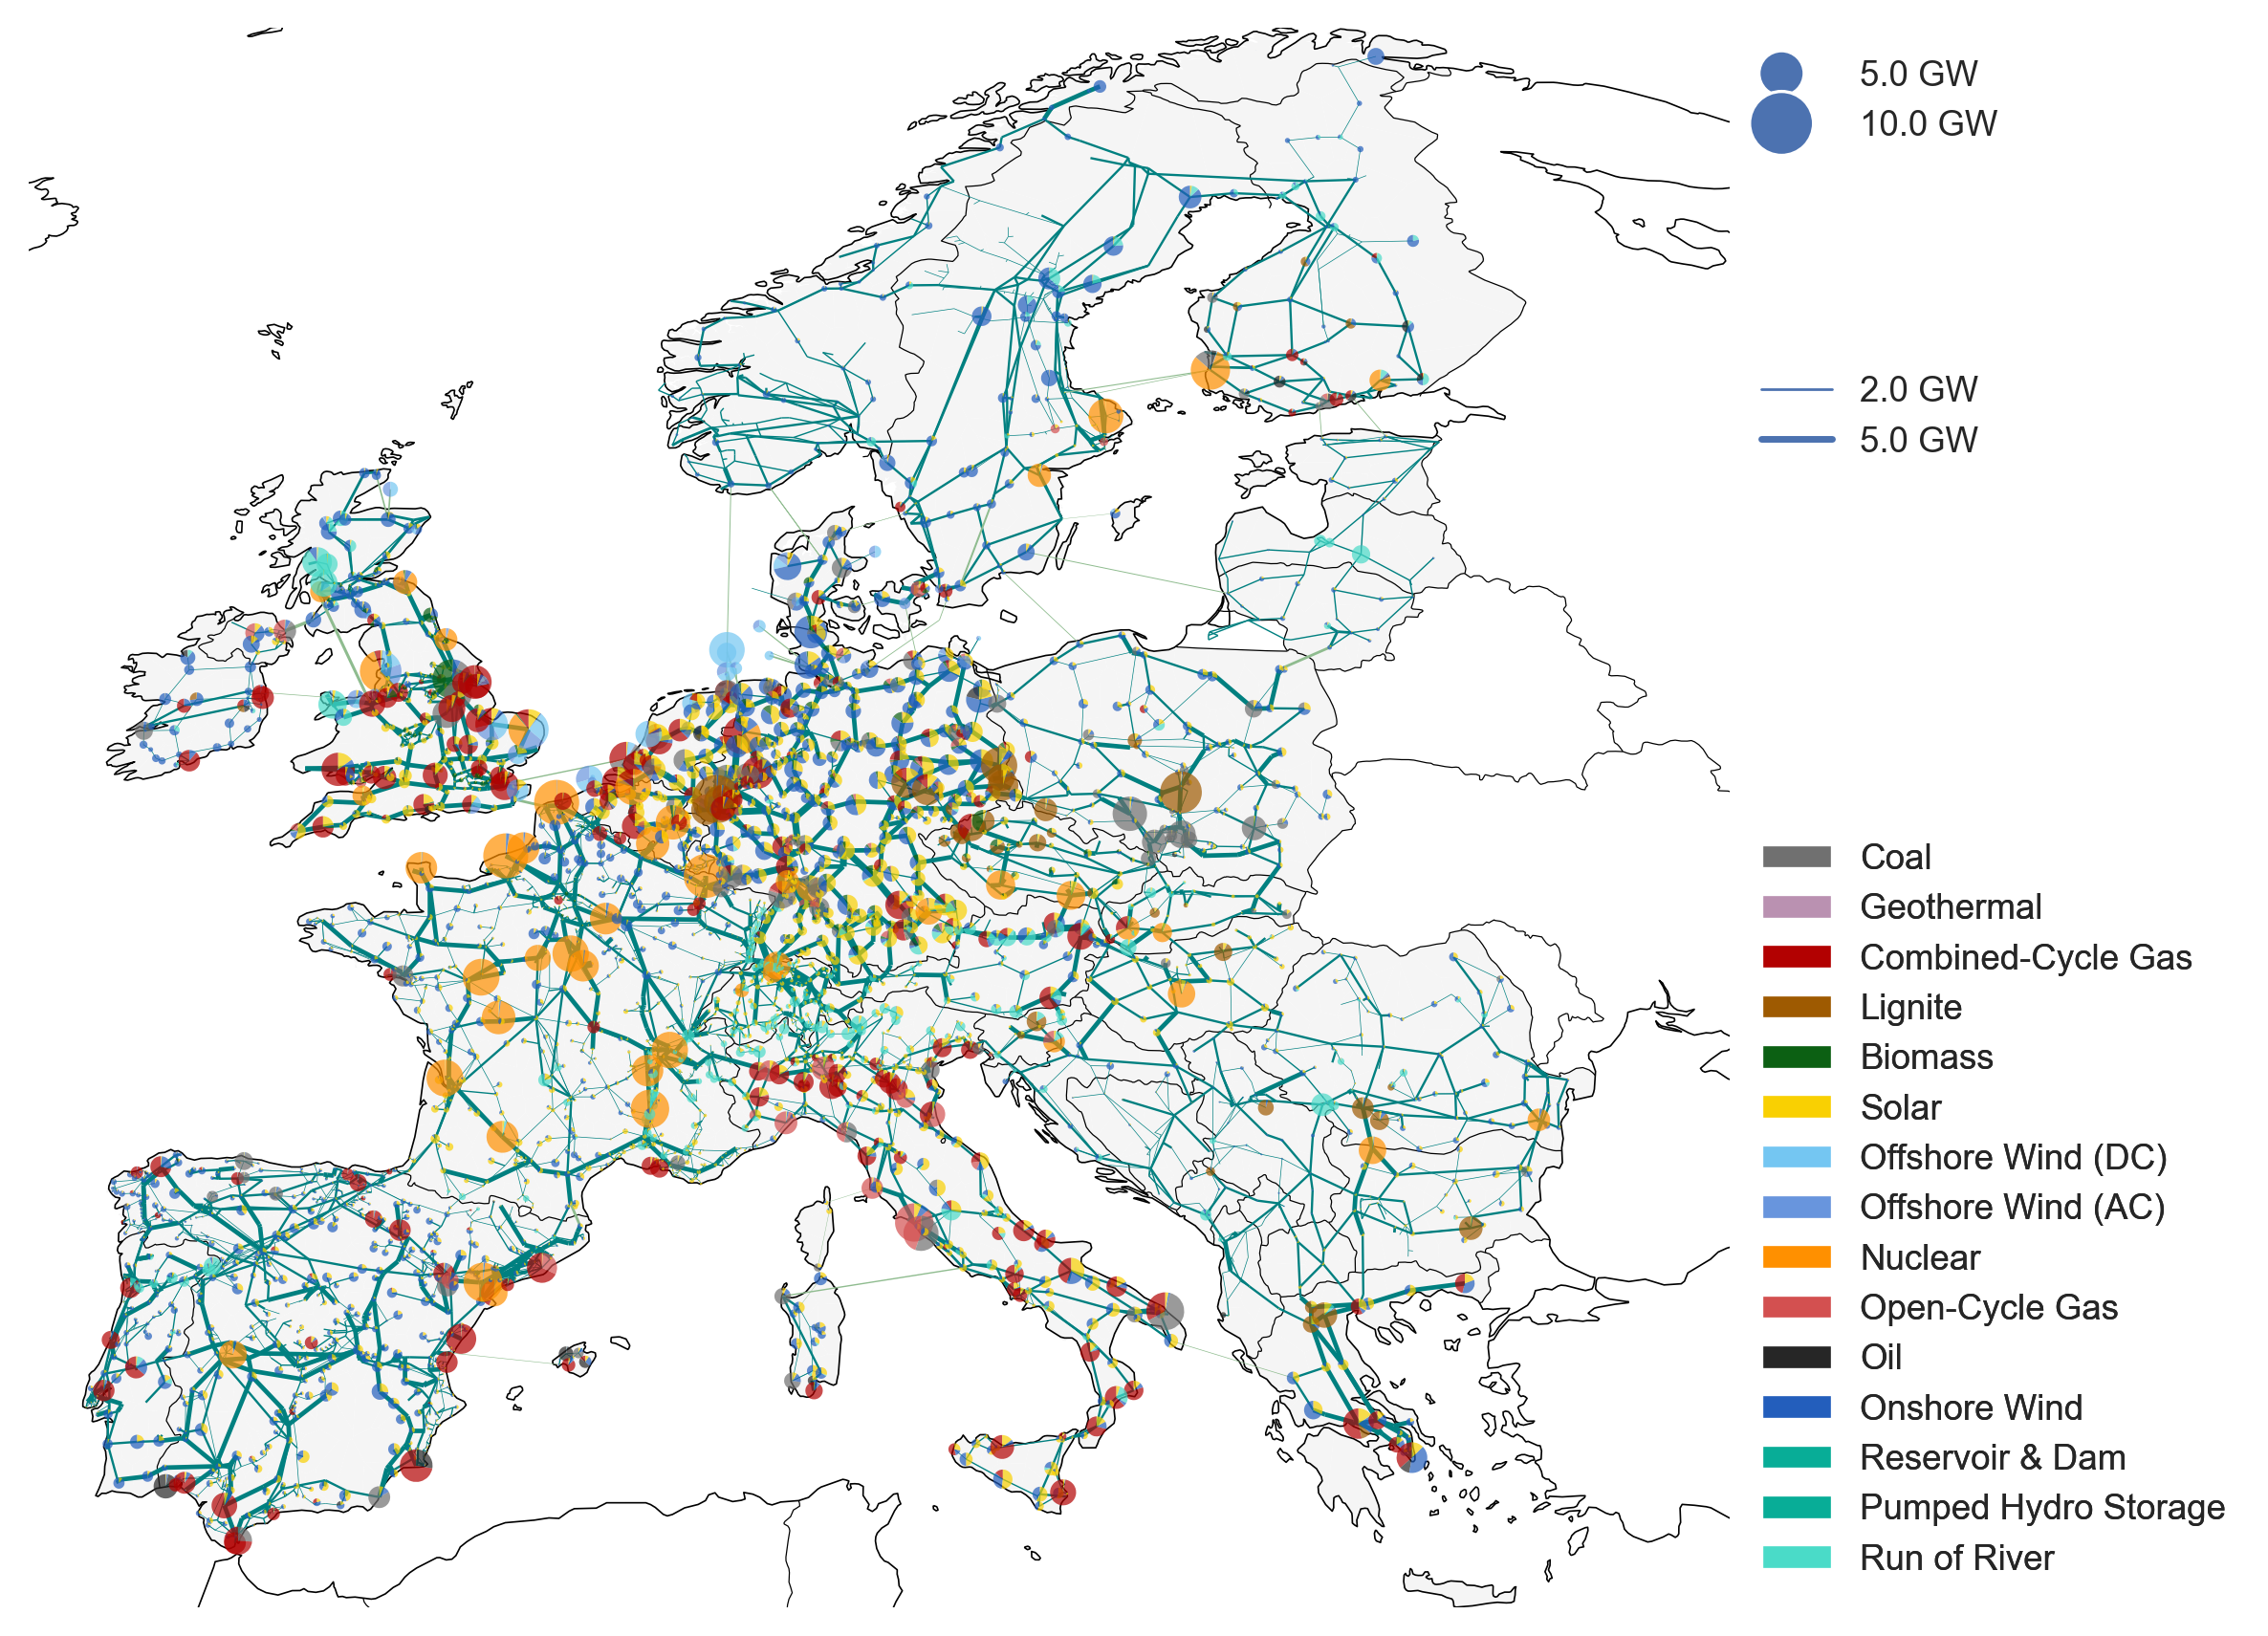
\includegraphics[width=1\textwidth]{other/pypsa_eur_elec}
%     \end{column}
%   \end{columns}

%   \source{\url{https://pypsa-eur.readthedocs.io}}
% \end{frame}

% \begin{frame}{Selection of planned model developments}
%   \footnotesize
%   \begin{columns}[T] % align columns
%     \begin{column}{.5\textwidth}
%         \begin{minipage}[t][.45\textheight]{\linewidth}
%             \begin{alertblock}{\textbf{Computational methods for uncertainties}}
%                 \begin{itemize}
%                   \item decomposition techniques
%                   \item large-scale stochastic optimisation
%                   \item \textbf{test robustness of system}
%                   \item using SMS++ framework
%                 \end{itemize}
%             \end{alertblock}
%         \end{minipage}
        
%         \vspace{-0.03\textheight} % separation between the boxes
        
%         \begin{minipage}[t][.45\textheight]{\linewidth}
%             \begin{alertblock}{\textbf{Industry transformation (FORECAST)}}
%               \begin{itemize}
%                 \item fuel and process switching
%                 \item industry relocation
%                 \item carbon sources and feedstocks
%                 \item data on stock \& investment cycles
%                 \item new technologies (oxyfuel cement, etc.)
%               \end{itemize}
%             \end{alertblock}
%         \end{minipage}
%     \end{column}
    
%     \begin{column}{.5\textwidth}
%         \begin{minipage}[t][.45\textheight]{\linewidth}
%             \begin{alertblock}{\textbf{Carbon management and biomass usage}}
%               \begin{itemize}
%                 \item \textbf{CO$_2$ network}
%                 \item \textbf{CO$_2$ sequestration potentials}
%                 \item circular carbon economy and recycling
%                 \item biomass usage options
%               \end{itemize}
%             \end{alertblock}
%         \end{minipage}
        
%         \vspace{-0.03\textheight} % separation between the boxes
        
%         \begin{minipage}[t][.45\textheight]{\linewidth}
%             \begin{alertblock}{\textbf{Global green fuel and material markets}}
%               \begin{itemize}
%                 \item \textbf{imports of green energy and materials}
%                 \item \textbf{effects on European infrastructure}
%                 \item restructuring of value chains
%                 \item risks (geopolitical, technological, etc.) \newline
%               \end{itemize}
%             \end{alertblock}
%         \end{minipage}
%     \end{column}
% \end{columns}
% \end{frame}

\section{Introduction \& Background}
\begin{frame}{Motivation: Recap 2030 policy targets}
  \footnotesize

  The EU has set ambitious targets for 2030, including the electricity, hydrogen and CO$_2$ infrastructure sector.

  \begin{columns}[T] % align columns
    % First column
    \begin{column}{.3\textwidth}
        \begin{minipage}[t][.45\textheight]{\linewidth}
            \begin{alertblock}{\textbf{55 \% emission reduction}}
                \begin{itemize}
                  \item \alert{Fit for 55}
                  \item Translating to an emission allowance of ca. 2 bn. t CO$_2$ p.a. in 2030
                  \item Covering the electricity, heat, industry, transport, buildings and agriculture sectors \newline
                \end{itemize}
                \vspace{0.06cm}
            \end{alertblock}
        \end{minipage}
    \end{column}
    
    % Second column
    \begin{column}{.34\textwidth}
        \begin{minipage}[t][.45\textheight]{\linewidth}
            \begin{exampleblock}{\textbf{10 Mt p.a. green H$_2$ production}}
                \begin{itemize}
                  \item \alert{REPowerEU}
                  \item Accelerating the transition away from fossil fuels (esp. Russian gas), enhancing energy security through renewables
                  \item Aligns with European Green Deal and targets scaling up renewable H$_2$ in hard-to-electrify-sectors
                \end{itemize}
            \end{exampleblock}
        \end{minipage}
    \end{column}

    % Third column
    \begin{column}{.3\textwidth}
        \begin{minipage}[t][.45\textheight]{\linewidth}
            \begin{exampleblock}{\textbf{50 Mt p.a. CO$_2$ sequestration}}
                \begin{itemize}
                  \item \alert{Net-Zero Industry Act}
                  \item Essential component in helping industries to reduce their net emissions
                  \item Provides means to capture unavoidable emissions from hard-to-abate sectors like cement, steel, chemicals, etc.
                \end{itemize}
            \end{exampleblock}
        \end{minipage}
    \end{column}
  \end{columns}

  \vspace{1.3cm}

\end{frame}

\begin{frame}{Motivation: PCI-PMI projects}
  \scriptsize
  \begin{columns}[T] % align columns
    % First column
    \begin{column}{.63\textwidth}
        \begin{minipage}[t][.45\textheight]{\linewidth}
            \begin{alertblock}{\textbf{What are PCI-PMI projects?}}
                \begin{itemize}
                  \setlength\itemsep{0.85em}
                  \item Projects of Common Interest (PCIs) are key \alert{cross-border infrastructure projects} that link the energy systems of EU countries
                  \item Projects of Mutual Interest (PMIs) include cooperations with countries outside the EU
                  \item Intend ``to help the EU achieve its \alert{energy policy and climate objectives}: affordable, secure and sustainable energy for all citizens and the long-term decarbonisation of the economy in accordance with the \alert{Paris Agreement}''
                  \item ``Potential overall benefits of the project must outweigh its costs'' 
                  \item Given their \alert{lighthouse character}, these projects are highly likely to be implemented. 
                  \item Large infrastructure projects (incl. PCI-PMI) are however commonly facing delays due to permitting, procurement bottlenecks, etc.
                \end{itemize}
            \end{alertblock}
        \end{minipage}
    \end{column}
    
    % Second column
    \begin{column}{.36\textwidth}
        \begin{minipage}[t][.45\textheight]{\linewidth}
            \begin{alertblock}{\textbf{Project map}}
              \centering
              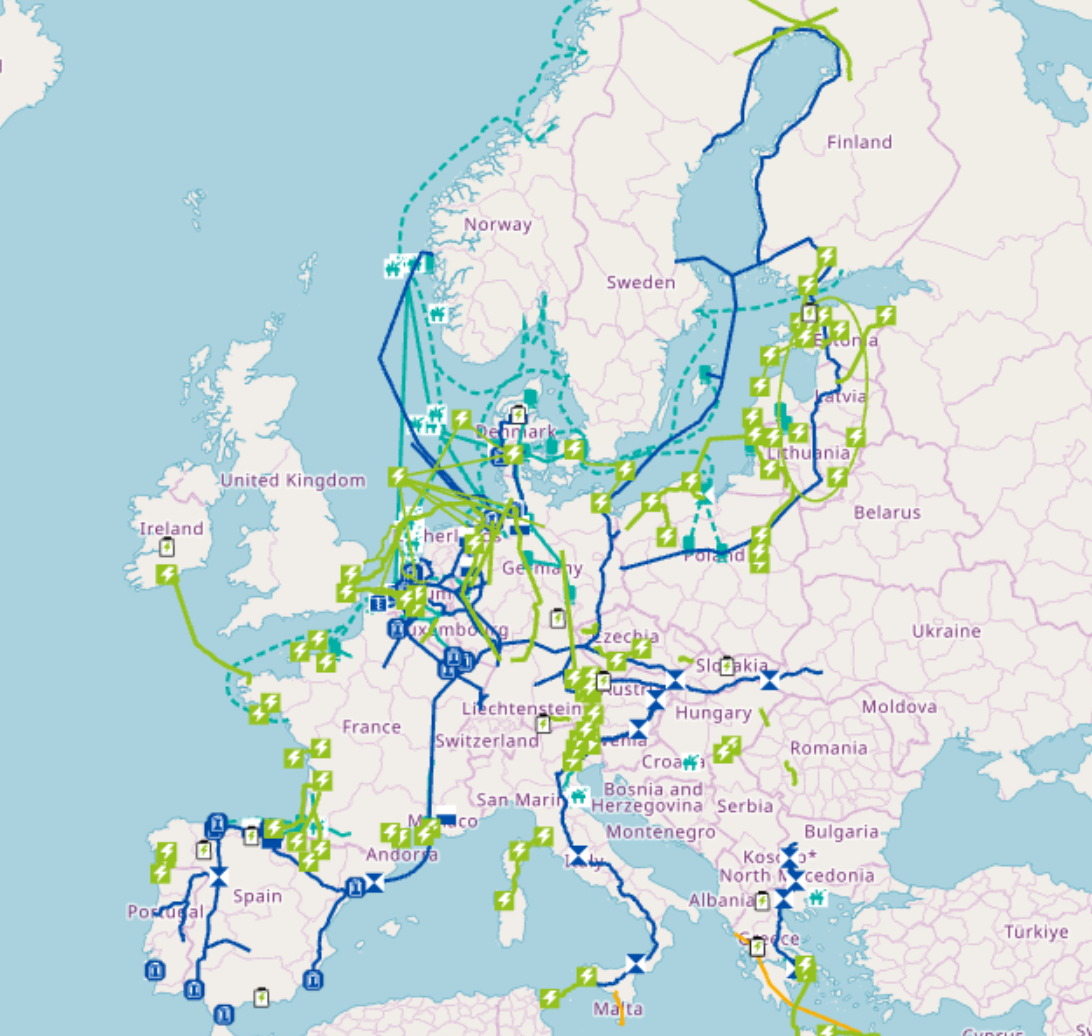
\includegraphics[width=1\textwidth]{pci_pmi_map}
            \end{alertblock}
        \end{minipage}
    \end{column}

  \end{columns}

  \vspace{2.2cm}

  \begin{enumerate}
    \item What is the impact of delay in PCI-PMI projects' realisation on the EU's policy targets for 2030?
    \item What are the costs associated with adhering to the EU policy targets, even if PCI-PMI projects are delayed? 
  \end{enumerate}

  \source{\url{https://energy.ec.europa.eu/topics/infrastructure_en} \\ and \url{https://ec.europa.eu/energy/infrastructure/transparency_platform/map-viewer}}

\end{frame}


\section{Methodology}

\begin{frame}{Model setup}
  \begin{columns}
    \begin{column}{0.55\textwidth}
      \footnotesize
      \begin{itemize}
        \setlength\itemsep{.8em}
        \item Including sectors \alert{power, heat, transport, industry, feedstock} and \alert{agriculture}
        \item \alert{Myopic optimisation} for 2030, 2040 and 2050
        \item \alert{Co-optimising} generation, transmission, storage, and power-to-X conversion
        \item Resolving 34 countries to \alert{99 regions} (NUTS mix) at \alert{4-hourly} temporal resolution on avg. (using tsam).
        \item Implementing \alert{PCI-PMI} HVAC, HVDC, hydrogen and carbon infrastructure projects as well as key GHG, \ce{H2} production, electrolyser capacity, and \ce{CO2} sequestration targets (next slide). Additional sequestration potential from \alert{depleted oil and gas fields} \cite{hofmannH2CO2Network2025}
        \item \alert{Regret analysis} approach based on 5 long-term scenario, 3 short-term scenarios, in total 60 model runs
      \end{itemize}
    \end{column}
    \begin{column}{0.45\textwidth}
      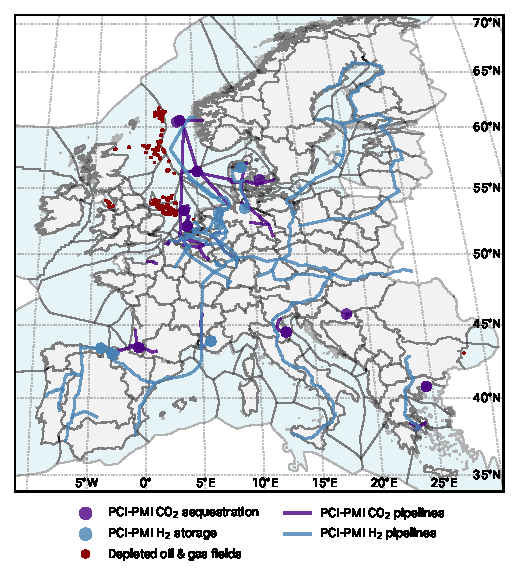
\includegraphics[width=1\textwidth]{map_adm_pcipmi}
    \end{column}
  \end{columns}
  \source{Own illustration based on data extracted from \url{https://ec.europa.eu/energy/infrastructure/transparency_platform/map-viewer}}
\end{frame}

\begin{frame}{Pathway for implemented long-term (LT) targets}
  \scriptsize
  \begin{tabularx}{\textwidth}{R{3.9cm}>{\centering\arraybackslash}X>{\centering\arraybackslash}X>{\centering\arraybackslash}X}
    \toprule
    \textbf{Planning horizon} & \textbf{2030} & \textbf{2040} & \textbf{2050} \\
    \midrule
    \textbf{Targets} & & & \\
    GHG emission reduction &  \SI{-55}{\percent} & \SI{-90}{\percent} & \SI{-100}{\percent} \\
    \ce{CO2} sequestration & 50 Mt p.a. & 150 Mt p.a. & 250 Mt p.a. \\
    Electrolytic \ce{H2} production & 10 Mt p.a. & 27.5 Mt p.a. & 45 Mt p.a. \\
    \ce{H2} electrolyser capacity & \SI{40}{GW} &  \SI{110}{GW} &  \SI{180}{GW} \\
    \bottomrule
  \end{tabularx}
  \scriptsize 
  \centering
  Model targets based on \cite{europeancommissionFit55Delivering2021,europeancommissionREPowerEUPlanCommunication2022,europeanparliamentRegulationEU20242024,europeancommissionCommunicationCommissionEuropean2024,europeancommission.directorategeneralforenergy.METIS3Study2023}

\end{frame}

\begin{frame}{Exogenous demand}
  \begin{figure}[htbp]
    \centering
    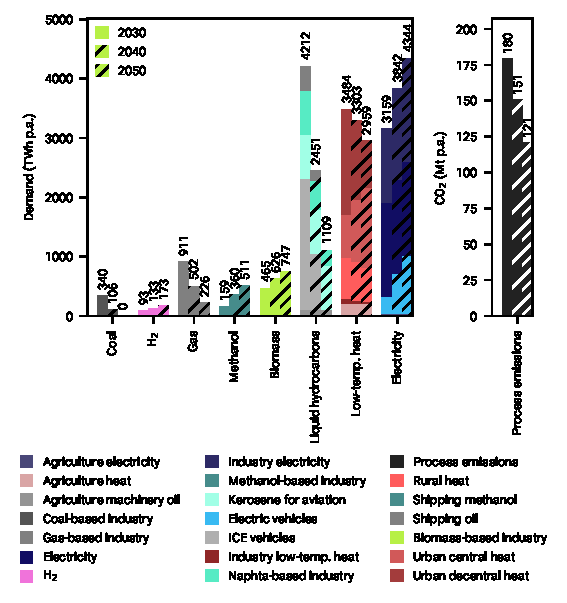
\includegraphics[width=0.52\textwidth]{exogenous_demand}
  \end{figure}
  \scriptsize
  asdf
\end{frame}


\begin{frame}{Long-term scenarios}
  \scriptsize
  \begin{tabularx}{\textwidth}{R{3.9cm}>{\centering\arraybackslash}X>{\centering\arraybackslash}X>{\centering\arraybackslash}X>{\centering\arraybackslash}X>{\centering\arraybackslash}X}
      \toprule
      \textbf{Long-term scenarios} & 
      \textbf{DI} & 
      \textbf{PCI} & 
      \textbf{PCI-n} & 
      \textbf{PCI-in} & 
      \textbf{CP} \\
      \midrule
      \textbf{\ce{CO2} sequestration} & & & & & \\
      Depleted oil \& gas fields* & $\blacksquare$ & $\blacksquare$ & $\blacksquare$ & $\blacksquare$ & $\blacksquare$ \\
      PCI-PMI seq. sites** & -- & $\blacksquare$ & $\blacksquare$ & $\blacksquare$ & $\blacksquare$ \\
      \midrule
      \textbf{\ce{H2} storage} & & & & & \\
      Endogenous build-out & $\blacksquare$ & $\blacksquare$ & $\blacksquare$ & $\blacksquare$ & $\blacksquare$ \\
      PCI-PMI storage sites & -- & $\blacksquare$ & $\blacksquare$ & $\blacksquare$ & $\blacksquare$ \\
      \midrule
      \textbf{\ce{CO2} pipelines} & & & & & \\
      to depleted oil \& gas fields & $\blacksquare$ & $\blacksquare$ & $\blacksquare$ & $\blacksquare$ & $\blacksquare$ \\
      to PCI-PMI seq. sites & -- & $\blacksquare$ & $\blacksquare$ & $\blacksquare$ & $\blacksquare$ \\
      \midrule
      \textbf{\ce{CO2} and \ce{H2} pipelines} & & & & & \\
      PCI-PMI & -- & $\blacksquare$ & $\blacksquare$ & $\blacksquare$ & $\blacksquare$ \\
      National build-out & -- & $\blacksquare$ & $\blacksquare$ & $\blacksquare$ & $\blacksquare$ \\
      International build-out & -- & -- & -- & $\blacksquare$ & $\blacksquare$ \\
      PCI-PMI extendable & -- & -- & -- & -- & $\blacksquare$ \\
      \bottomrule
  \end{tabularx}
  \vspace{0.5em}
  \centering
  {\scriptsize $\blacksquare$ enabled \quad -- disabled \quad * approx. 286 Mt p.a. \quad ** approx. 114 Mt p.a.}
\end{frame}

\begin{frame}{Regret-matrix setup}
  \scriptsize
  \begin{tabularx}{\textwidth}{R{3.9cm}>{\centering\arraybackslash}X>{\centering\arraybackslash}X>{\centering\arraybackslash}X}
    \toprule
    \textbf{Short-term} & \textbf{Reduced targets} & \textbf{Delayed pipelines} & \textbf{No pipelines} \\
    \midrule
    \textbf{Long-term scenarios} & & & \\
    Decentral Islands (\textbf{DI}) & $\blacksquare$ & -- & -- \\
    PCI-PMI (\textbf{PCI}) & $\blacksquare$ & $\blacksquare$ & $\blacksquare$ \\
    PCI-PMI nat. (\textbf{PCI-n}) & $\blacksquare$ & $\blacksquare$ & $\blacksquare$\\
    PCI-PMI internat. (\textbf{PCI-in}) & $\blacksquare$ & $\blacksquare$ & $\blacksquare$ \\
    Central Planning (\textbf{CP}) & $\blacksquare$ & $\blacksquare$ & $\blacksquare$ \\
    \midrule
    \textbf{Targets} & & & \\
    GHG emission reduction &  $\blacksquare$ &  $\blacksquare$ &  $\blacksquare$ \\
    \ce{CO2} sequestration &  -- &  $\blacksquare$ &  $\blacksquare$ \\
    Electrolytic \ce{H2} production &  -- &  $\blacksquare$ &  $\blacksquare$ \\
    \ce{H2} electrolysers &  -- &  $\blacksquare$ &  $\blacksquare$ \\
    \midrule
    \textbf{\ce{CO2} + \ce{H2} infrastructure} & & & \\
    \ce{CO2} sequestration sites & $\blacksquare$ &  $\blacksquare$ &  $\blacksquare$ \\
    \ce{CO2} pipelines to seq. site & $\blacksquare$ &  $\blacksquare$ &  $\blacksquare$ \\
    \ce{CO2} pipelines & $\blacksquare$ &  $\square$ &  -- \\
    \ce{H2} pipelines & $\blacksquare$ &  $\square$ &  -- \\
    \bottomrule
  \end{tabularx}
  \centering
  \scriptsize $\blacksquare$ enabled \quad $\square$ delayed by one period \quad -- disabled

\end{frame}

\begin{frame}{LT --- PCI: 2030 regional \ce{H2}, \ce{CO2} balances and transport}
  \centering
  \begin{columns}
    \begin{column}{0.5\textwidth}
      \footnotesize
      \begin{figure}
        \centering
        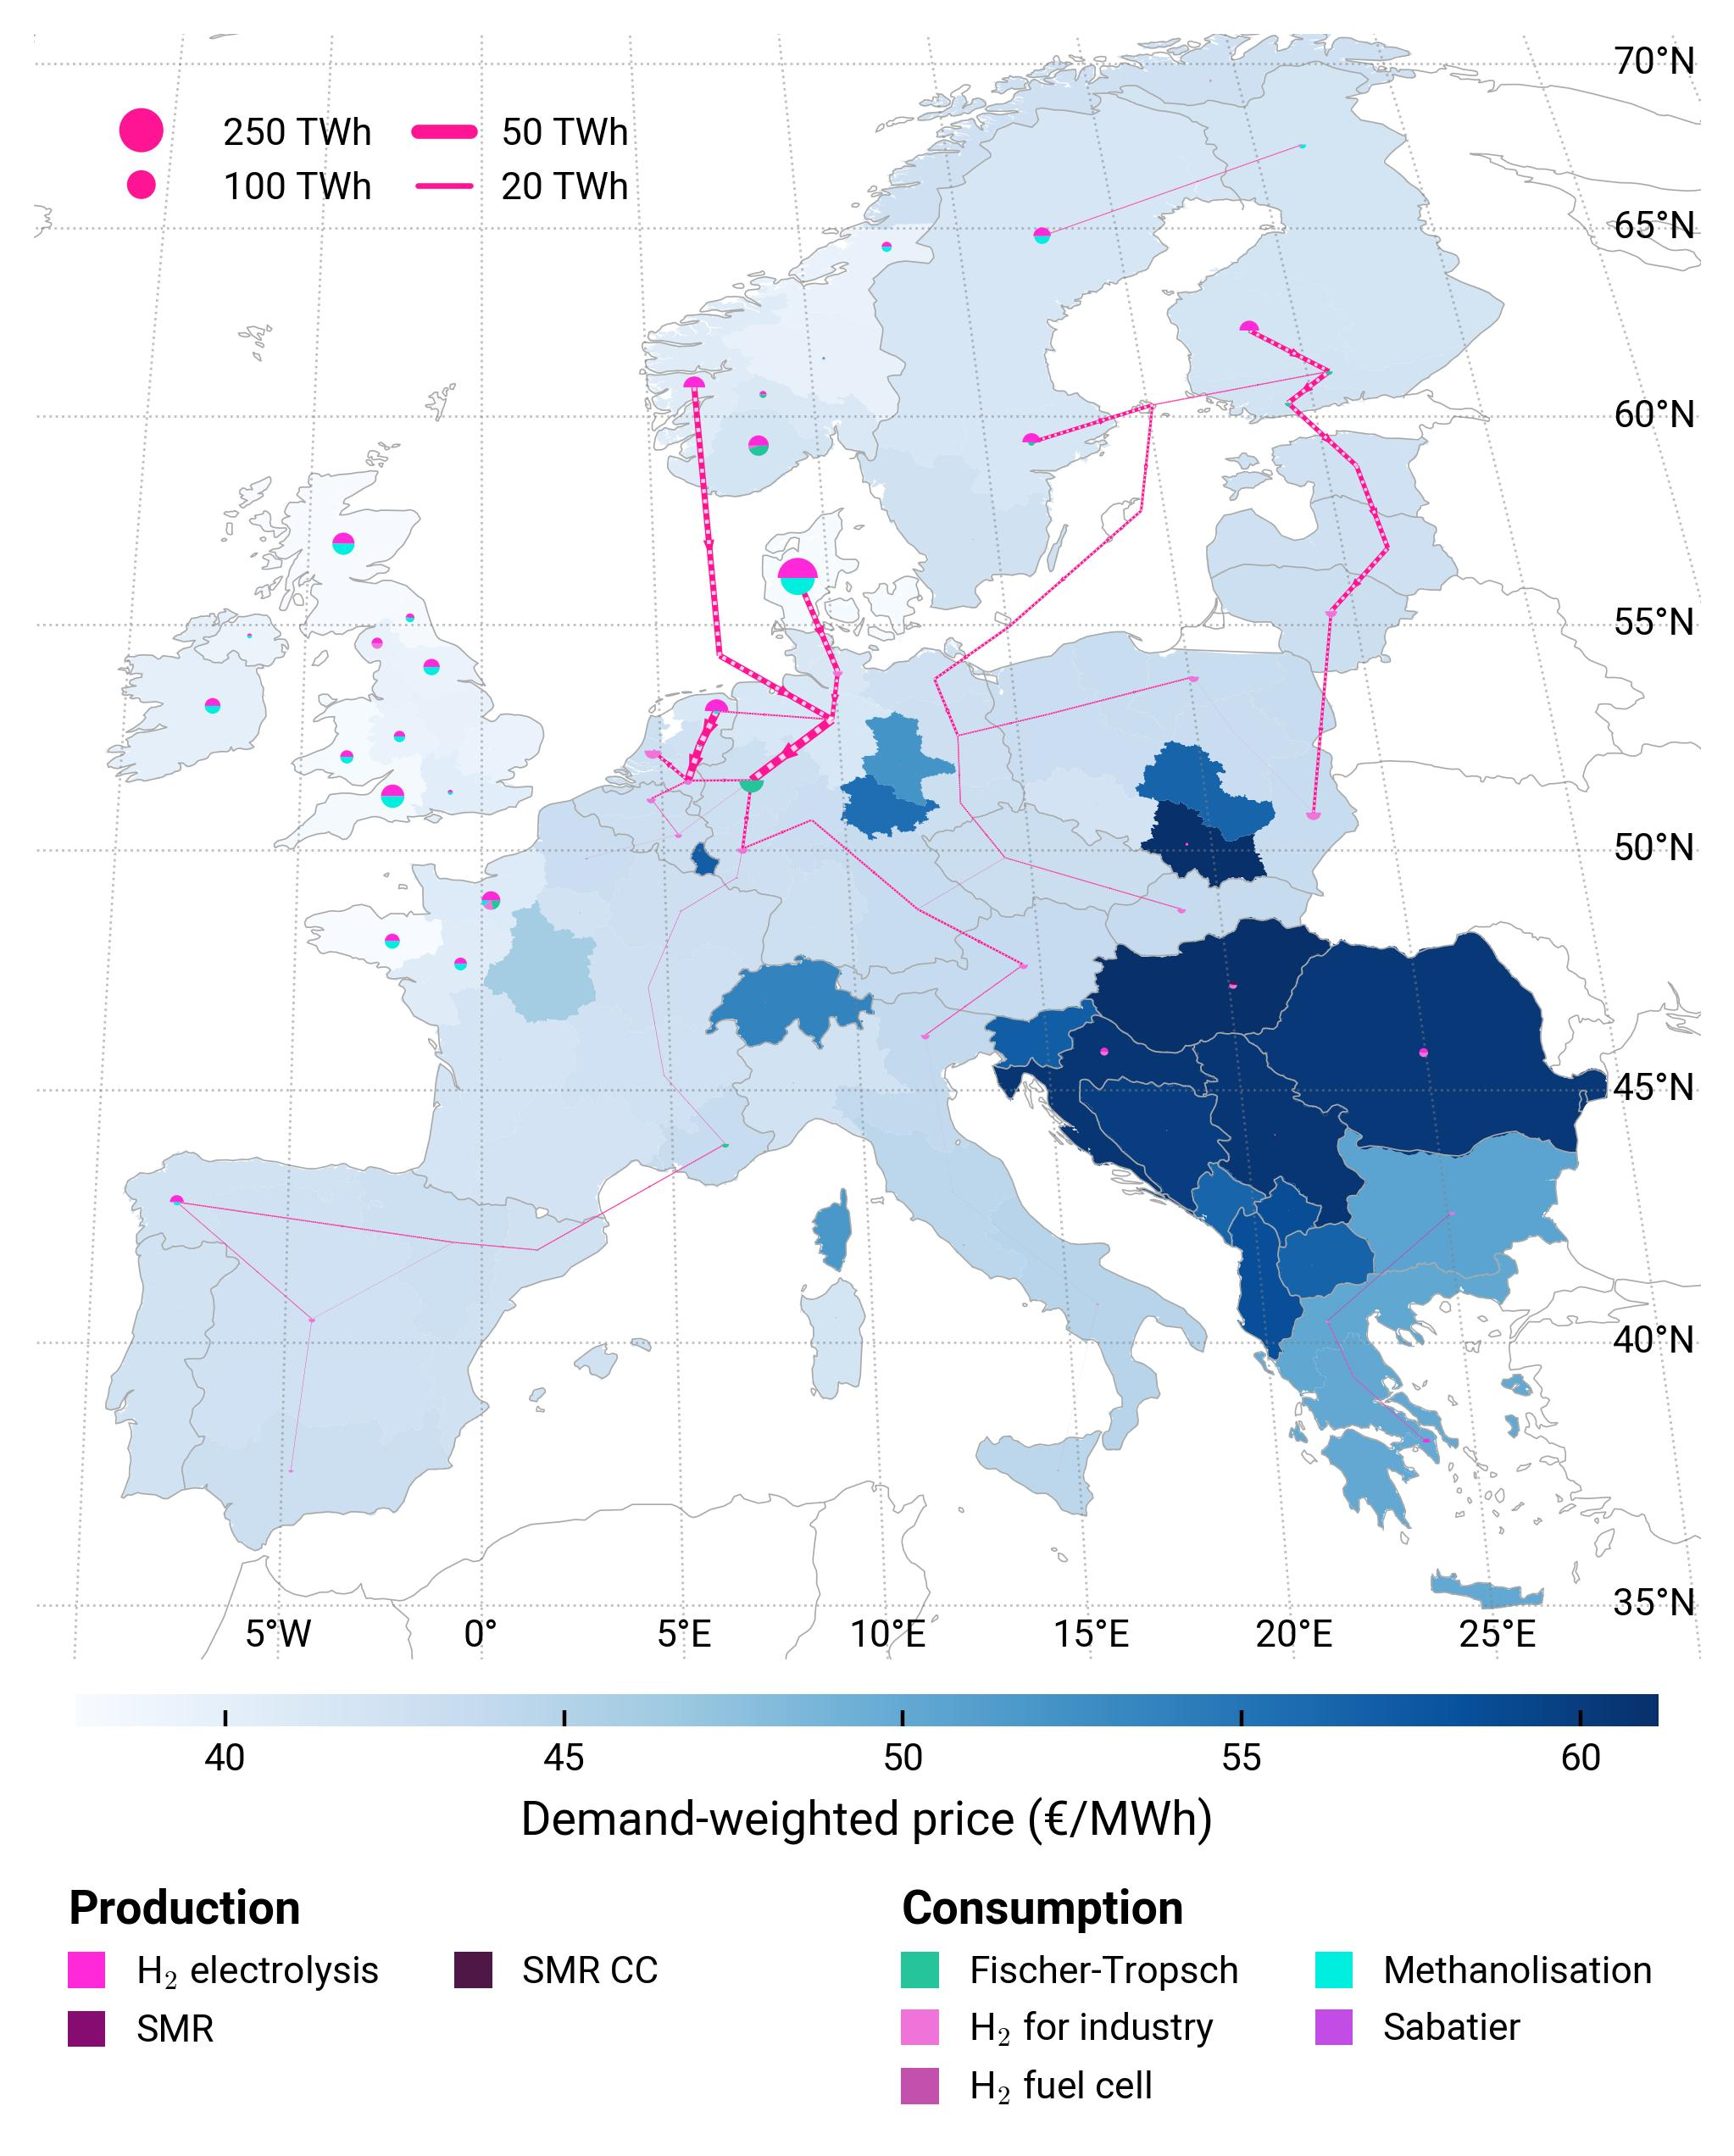
\includegraphics[width=0.8\textwidth]{maps/pcipmi/base_s_adm___2030-balance_map_H2}
      \end{figure}
    \end{column}
    \begin{column}{0.5\textwidth}
      \begin{figure}
        \centering
        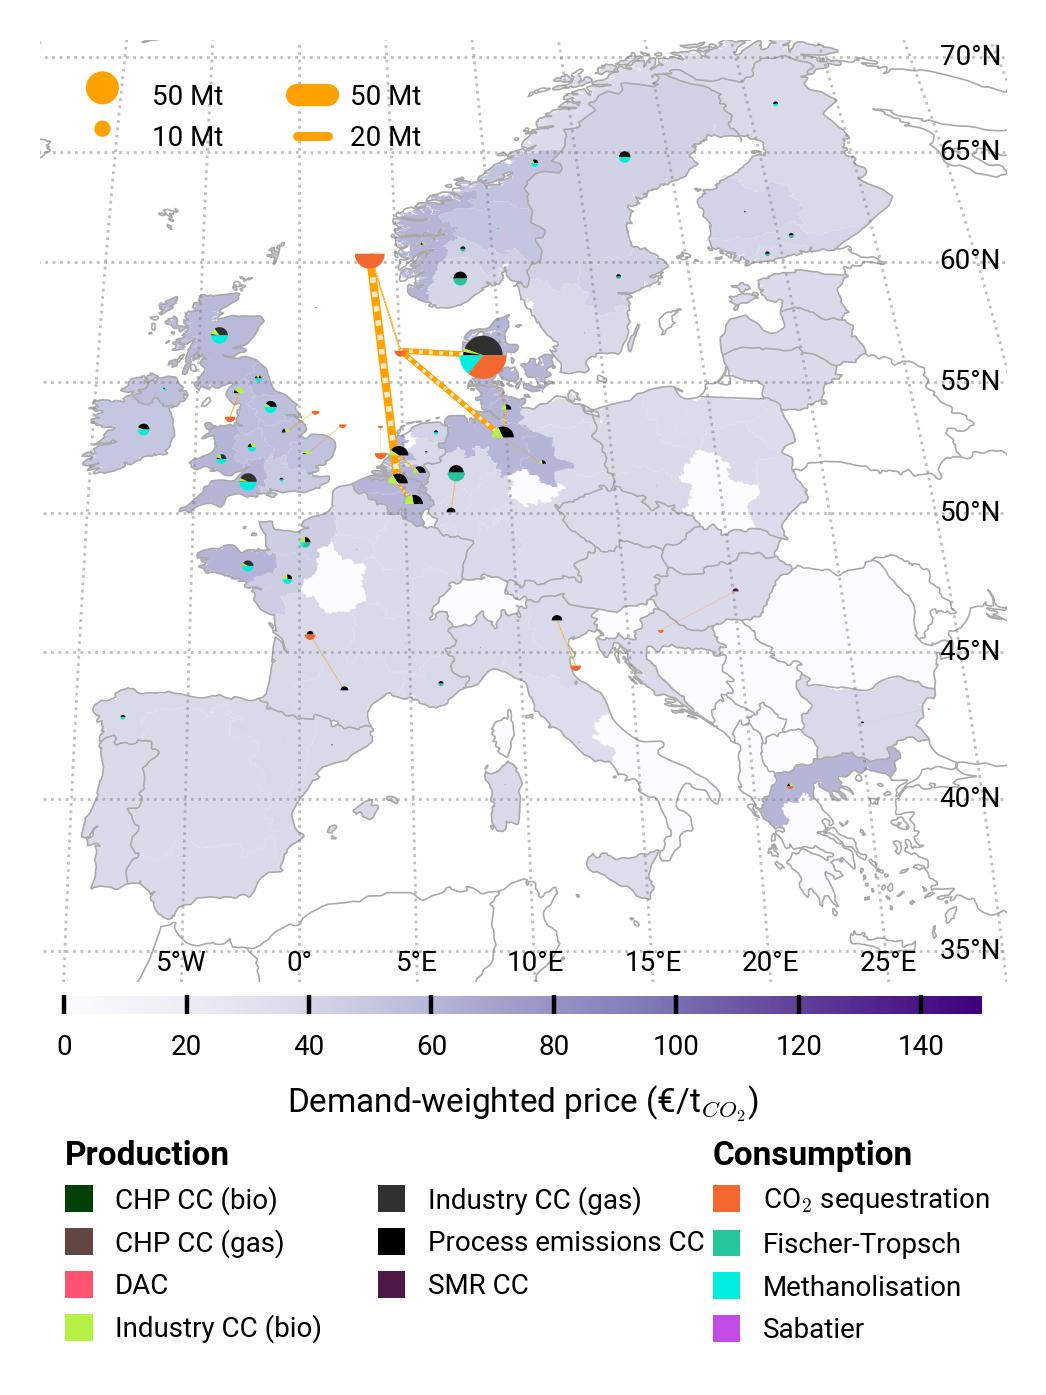
\includegraphics[width=0.8\textwidth]{maps/pcipmi/base_s_adm___2030-balance_map_co2_stored}
      \end{figure}
    \end{column}
  \end{columns}
  \source{Own illustration.}
\end{frame}

\begin{frame}{LT --- PCI: 2040 regional \ce{H2}, \ce{CO2} balances and transport}
  \centering
  \begin{columns}
    \begin{column}{0.5\textwidth}
      \footnotesize
      \begin{figure}
        \centering
        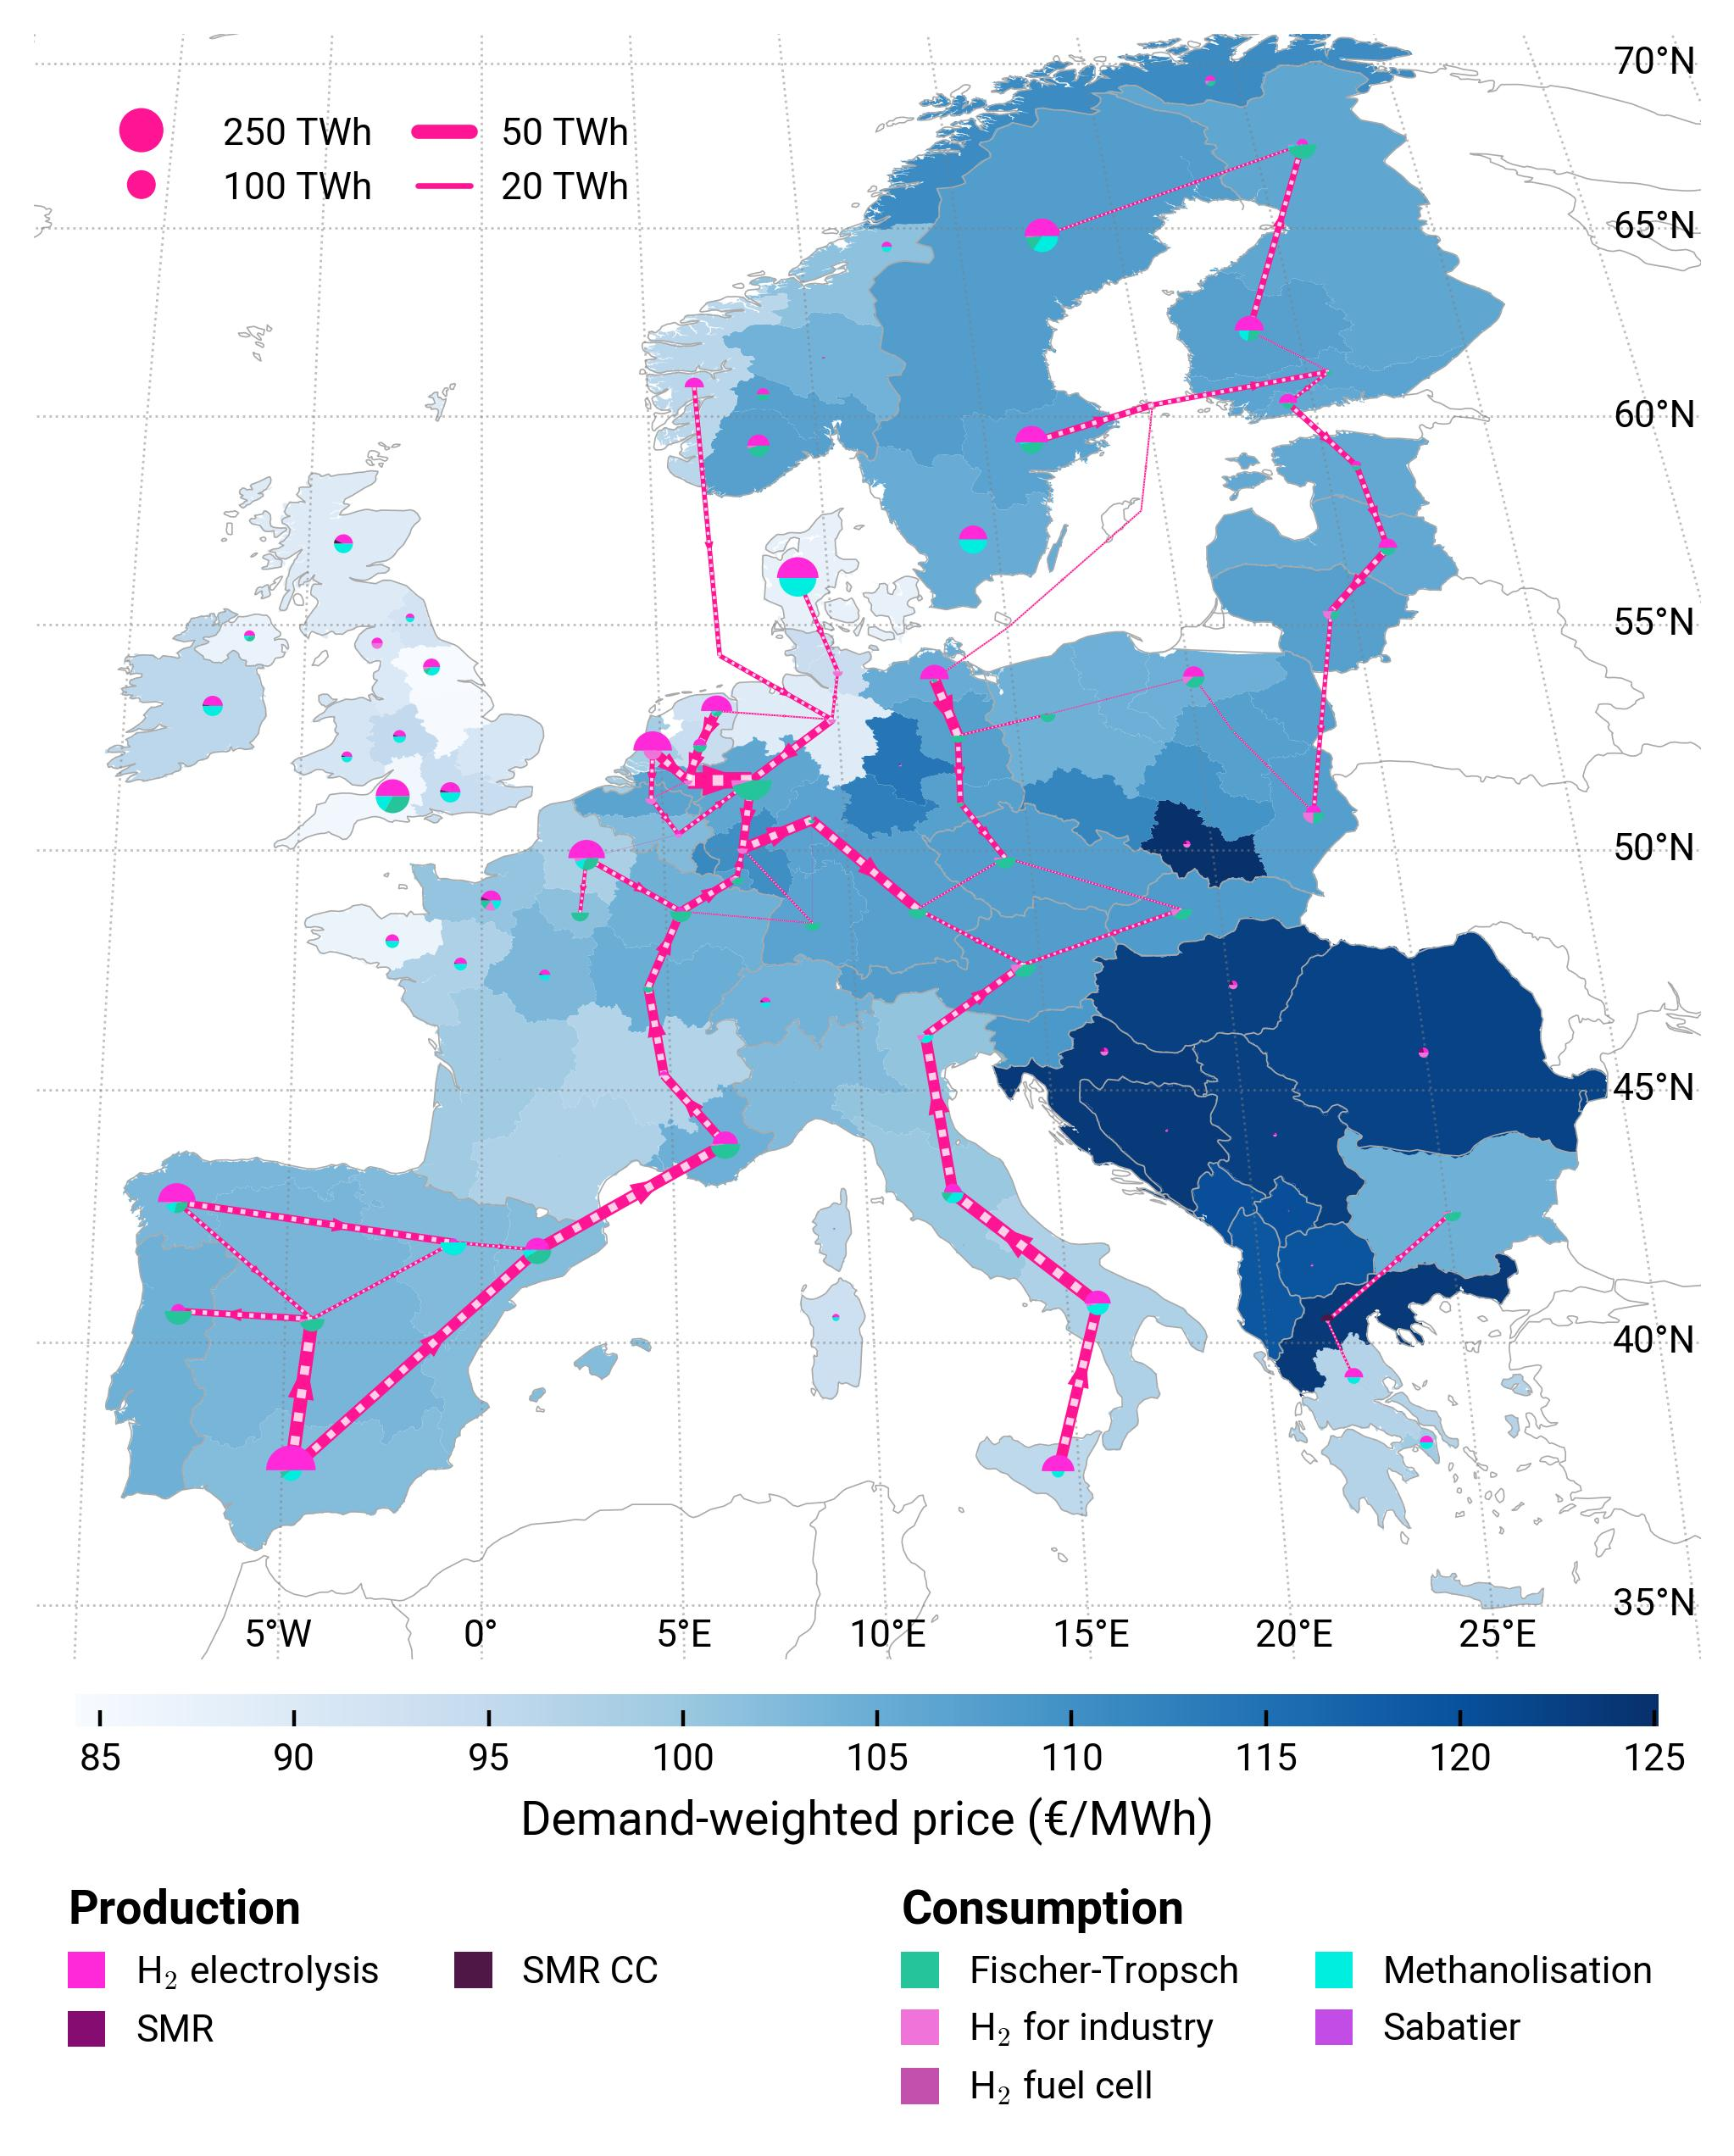
\includegraphics[width=0.8\textwidth]{maps/pcipmi/base_s_adm___2040-balance_map_H2}
      \end{figure}
    \end{column}
    \begin{column}{0.5\textwidth}
      \begin{figure}
        \centering
        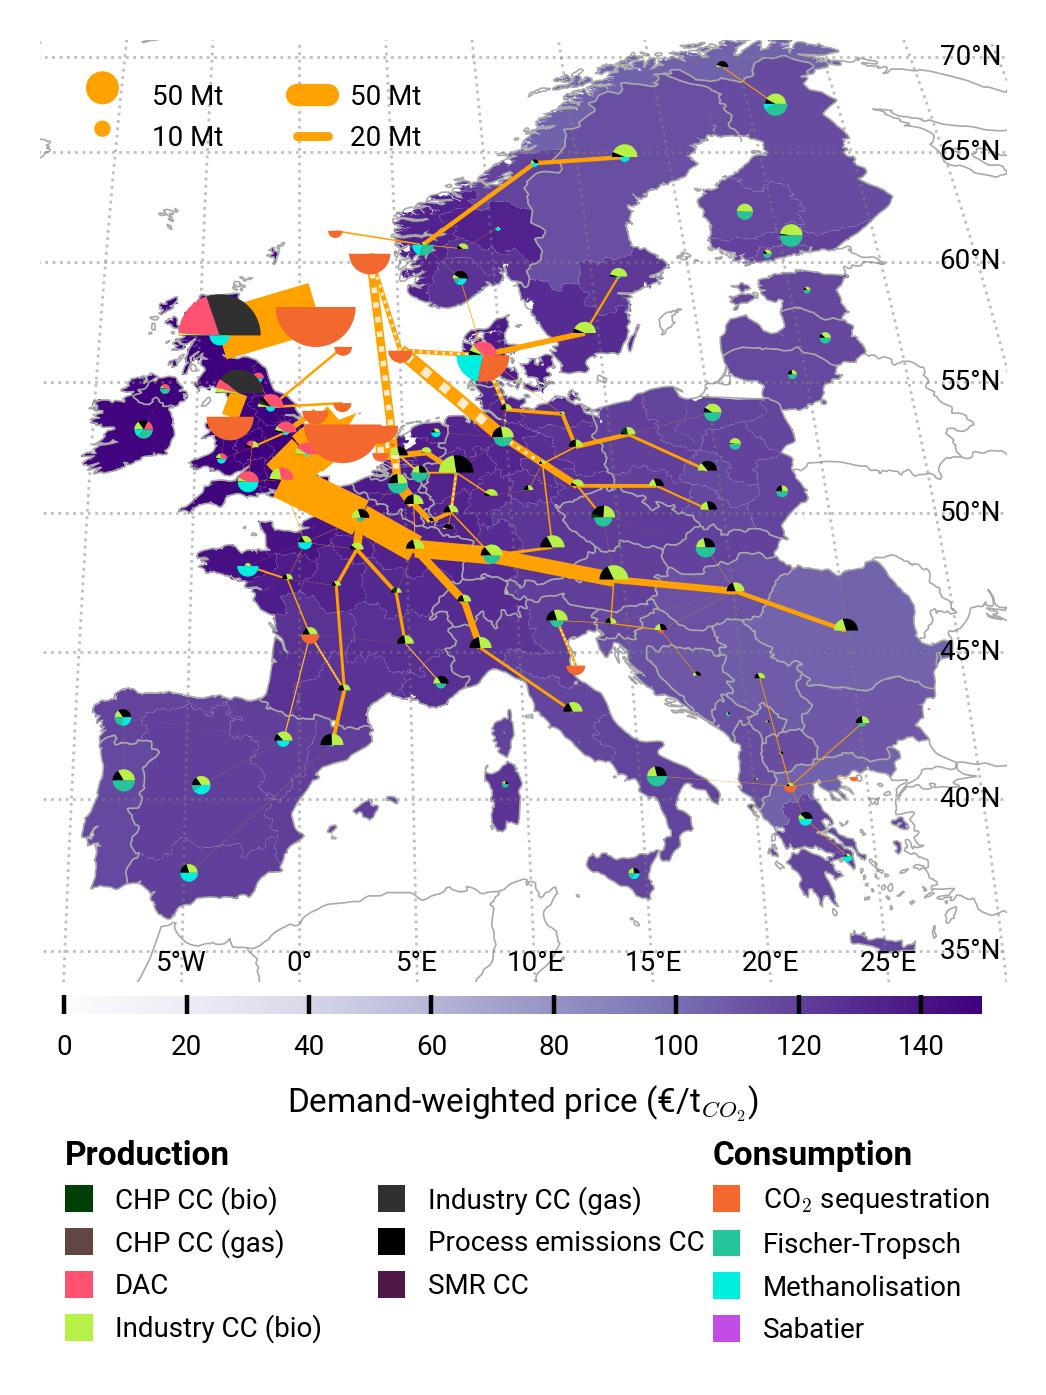
\includegraphics[width=0.8\textwidth]{maps/pcipmi/base_s_adm___2040-balance_map_co2_stored}
      \end{figure}
    \end{column}
  \end{columns}
  \source{Own illustration.}
\end{frame}

\begin{frame}{LT --- PCI: 2050 regional \ce{H2}, \ce{CO2} balances and transport}
  \centering
  \begin{columns}
    \begin{column}{0.5\textwidth}
      \footnotesize
      \begin{figure}
        \centering
        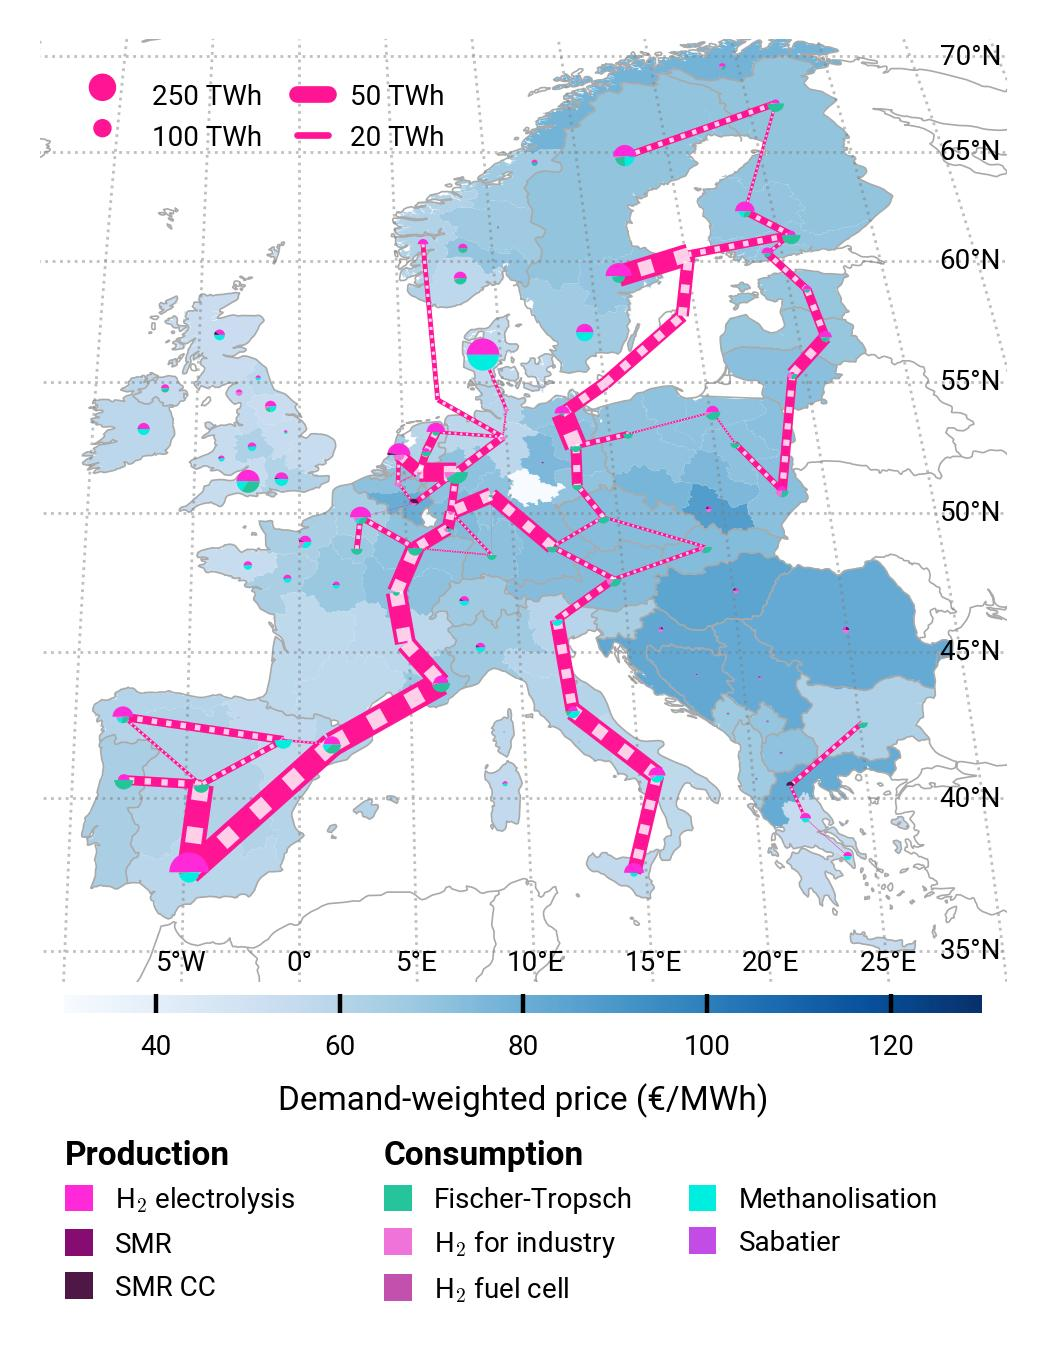
\includegraphics[width=0.8\textwidth]{maps/pcipmi/base_s_adm___2050-balance_map_H2}
      \end{figure}
    \end{column}
    \begin{column}{0.5\textwidth}
      \begin{figure}
        \centering
        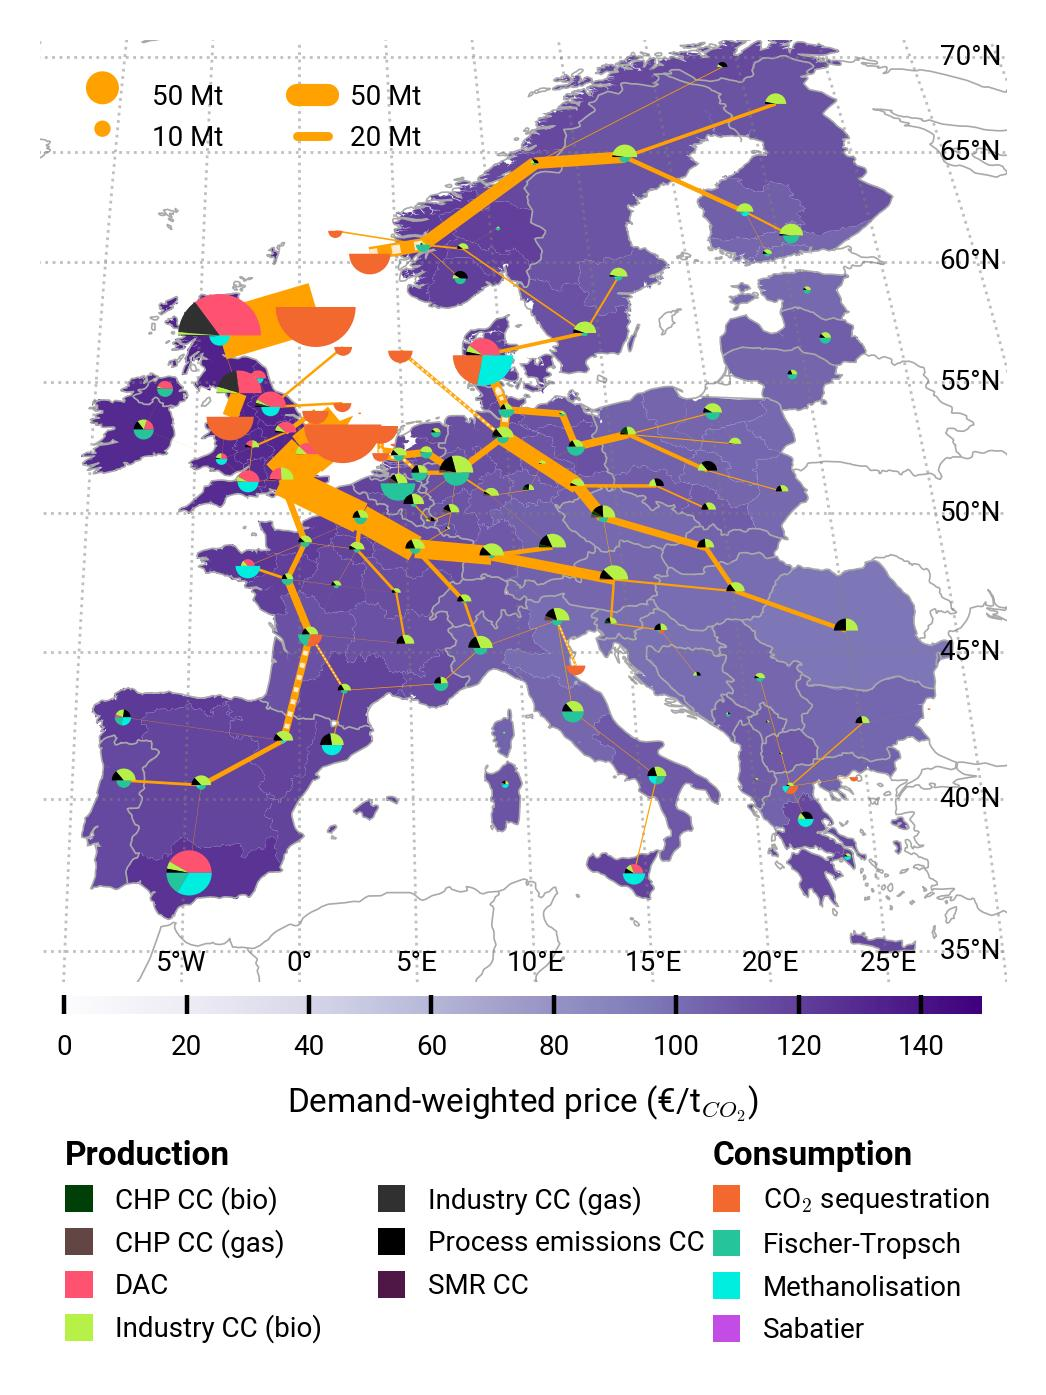
\includegraphics[width=0.8\textwidth]{maps/pcipmi/base_s_adm___2050-balance_map_co2_stored}
      \end{figure}
    \end{column}
  \end{columns}
  \source{Own illustration.}
\end{frame}


\section{Results \& Discussion}
\begin{frame}{LT --- Total system costs}
  \begin{figure}[htbp]
    \centering
    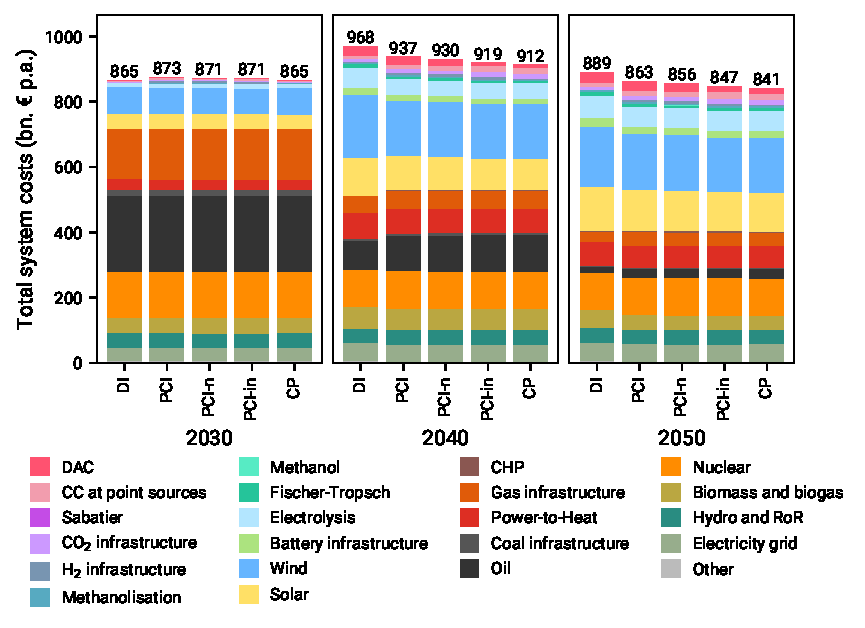
\includegraphics[width=0.65\textwidth]{costs_overview}
    % \caption{Total annual system costs (CAPEX + OPEX) by technology group.}
  \end{figure}
\end{frame}

\begin{frame}{LT --- \ce{CO2} balances}
  \begin{figure}[htbp]
    \centering
    \includegraphics[width=0.75\textwidth]{delta_balances_dac}
  \end{figure}
\end{frame}

\begin{frame}{LT --- \ce{CO2} balances: Direct Air Capture (DAC) utilisation}
  \begin{figure}[htbp]
    \centering
    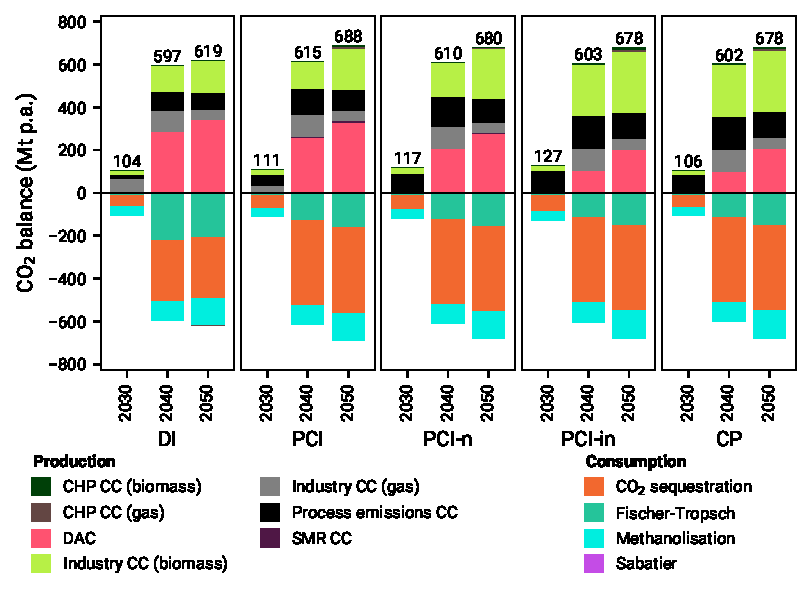
\includegraphics[width=0.65\textwidth]{balances_overview_co2 stored}
    % \caption{Total annual system costs (CAPEX + OPEX) by technology group.}
  \end{figure}
\end{frame}

\begin{frame}{LT --- \ce{H2} balances}
  \begin{figure}[htbp]
    \centering
    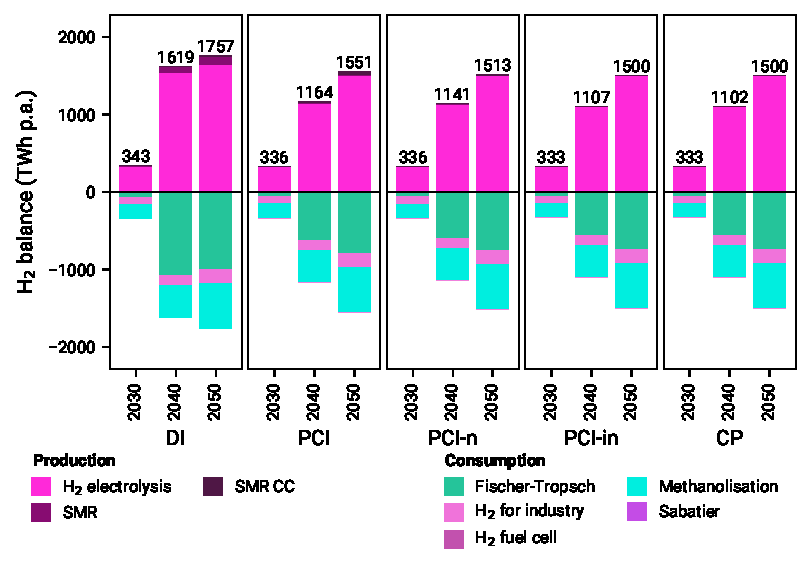
\includegraphics[width=0.65\textwidth]{balances_overview_H2}
    % \caption{Total annual system costs (CAPEX + OPEX) by technology group.}
  \end{figure}
\end{frame}

\begin{frame}{Regret matrix}
  \begin{figure}[htbp]
    \centering
    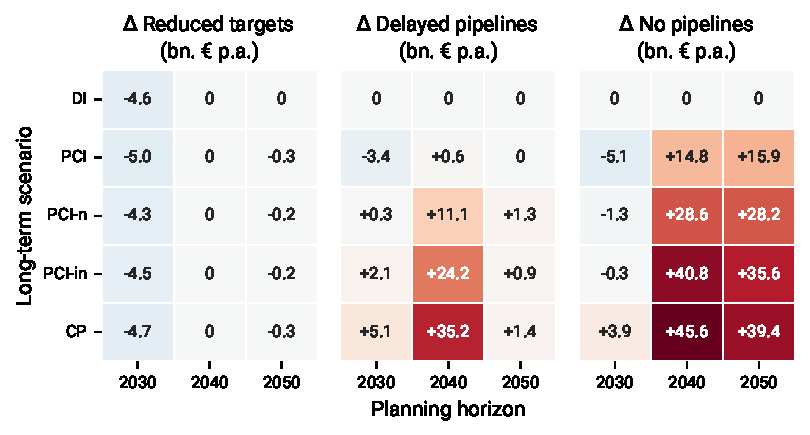
\includegraphics[width=0.65\textwidth]{regret_matrix}
  \end{figure}
  \scriptsize
  \centering
  Regret terms are calculated by subtracting system costs of long-term scenarios (rows) from short-term scenarios (columns). Positive values reflect higher costs in the short-term scenarios compared to the long-term ones.
\end{frame}

\begin{frame}{Value of PCI-PMI projects in the long run}
  \begin{figure}[htbp]
    \centering
    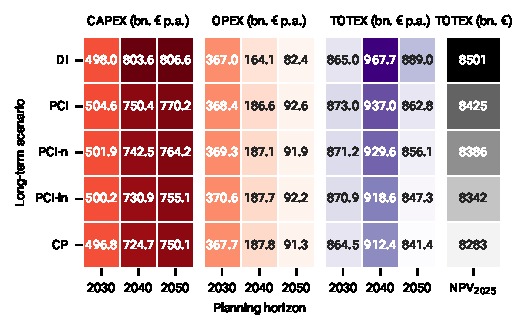
\includegraphics[width=0.65\textwidth]{totex_heatmap}
  \end{figure}
\end{frame}


\section{Conclusion}
\begin{frame}{Conclusion}
  \footnotesize
  \begin{enumerate}
    \setlength\itemsep{0.3em}
    \item PCI-PMI projects have a positive impact on total system costs and are likely a no-regret investment based on our results (though not perfectly cost-optimal compared to theoretical \textit{CP} scenario).
    \item Additional cost savings can be unlocked with single, strategically placed pipelines to connect additional \ce{H2} production sites and \ce{CO2} point sources to the pipeline network.
    \item Further, the success of large-scale investment projects is largely driven by political support, public acceptance, which is especially given for PCI-PMI projects.
    \item \ce{H2} pipelines projects help distribute more affordable green H$_2$ from northern and south-western Europe to high-demand regions in central Europe; ii) \ce{CO2} transport and storage projects help decarbonising the industry by connecting major industrial sites and their process emissions to offshore sequestration sites in the North Sea (Denmark, Norway, and the Netherlands).
    \item Pipelines basically serve as a tool to hedge risks of overbuilding solar and wind generation capacities and reduce excessive reliance on single carbon capture technologies like DAC and carbon capture at point sources $\rightarrow$ confirms previous findings of \cite{hofmannH2CO2Network2025}.
    \item Overall, PCI-PMI projects including additional pipeline build-outs allow a lower-cost and less technology-dependent transition towards a decarbonised system compared to a system without any pipeline infrastructure. They support achieving the EUs ambitious policy targets in the long run.
  \end{enumerate}

\end{frame}


% \begin{frame}[allowframebreaks]{References (excerpt)}
\begin{frame}{References (excerpt)}
  \begingroup
  \renewcommand*{\bibfont}{\scriptsize}
  \printbibliography
  \endgroup
\end{frame}

\begin{frame}
  \setbeamercolor{background canvas}{bg=red}
  \centering
  \fcolorbox{white}{tub-red}{\parbox[c][0.9\textheight][c]{\textwidth}{%
      \centering \color{white}\Large{\textbf{Thank you.}} \\ 
      \scriptsize
      \vspace{0.5cm}
      \href{https://github.com/pypsa/pypsa-eur}{\textcolor{white}{$\hookrightarrow$ github.com/pypsa/pypsa-eur}} \\
      \vspace{0.5cm}
      Department of\\\textbf{Digital Transformation in Energy Systems (ENSYS)} \\
      \vspace{0.5cm}
      \textbf{Bobby Xiong}\\
      \href{mailto:xiong@tu-berlin.de}{\textcolor{white}{$\hookrightarrow$ xiong@tu-berlin.de}} \\
      \href{https://github.com/bobbyxng}{\textcolor{white}{$\hookrightarrow$ github.com/bobbyxng}} \\
  }}
\end{frame}

% Appendix
\section{Appendix}

\begin{frame}
  \setbeamercolor{background canvas}{bg=red}
  \centering
  \fcolorbox{white}{tub-red}{\parbox[c][0.9\textheight][c]{\textwidth}{%
      \centering \color{white}\Large{\textbf{Appendix}}
  }}
\end{frame}

\begin{frame}{LT --- Installed capacities}
  \begin{figure}[htbp]
    \centering
    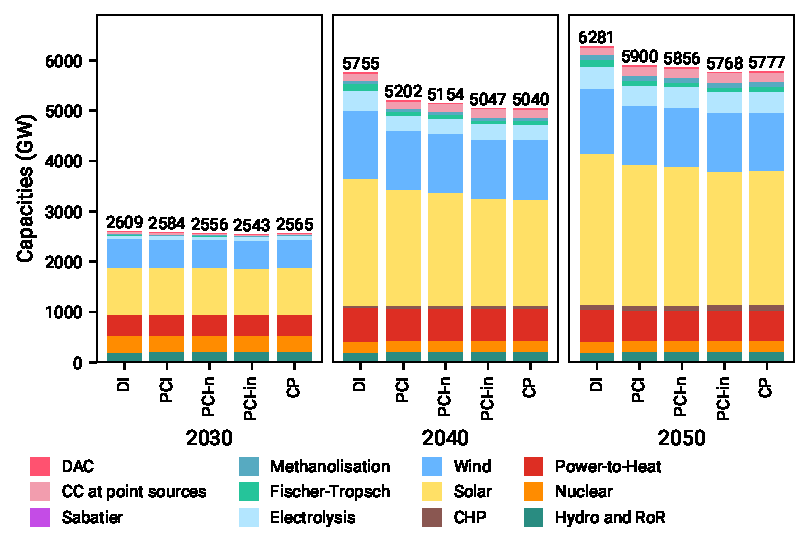
\includegraphics[width=0.65\textwidth]{capacities_overview}
  \end{figure}
\end{frame}

\begin{frame}{ST --- Delta system costs}
  \begin{figure}[htbp]
    \centering
    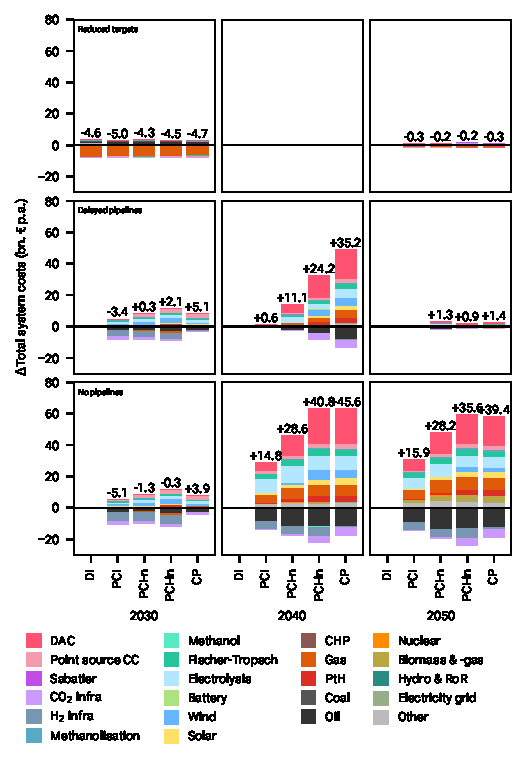
\includegraphics[width=0.53\textwidth]{costs_overview_extended}
  \end{figure}
\end{frame}

\begin{frame}{ST --- Delta capacities}
  \begin{figure}[htbp]
    \centering
    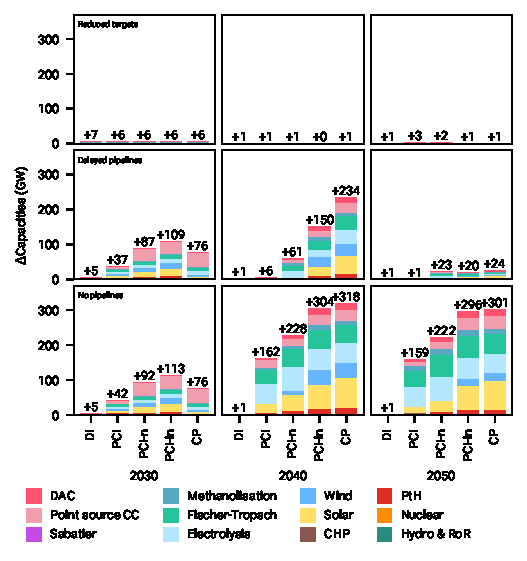
\includegraphics[width=0.49\textwidth]{capacities_overview_extended}
  \end{figure}
\end{frame}

\begin{frame}{ST --- Delta balances \ce{CO2}}
  \begin{figure}[htbp]
    \centering
    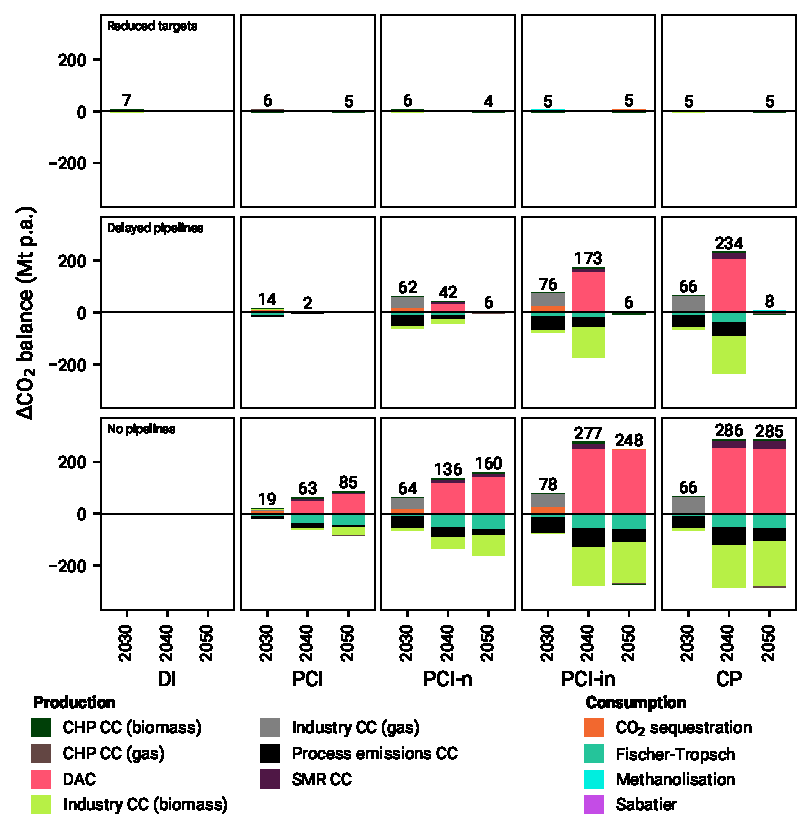
\includegraphics[width=0.49\textwidth]{balances_overview_extended_co2 stored}
  \end{figure}
\end{frame}

\begin{frame}{ST --- Delta balances \ce{H2}}
  \begin{figure}[htbp]
    \centering
    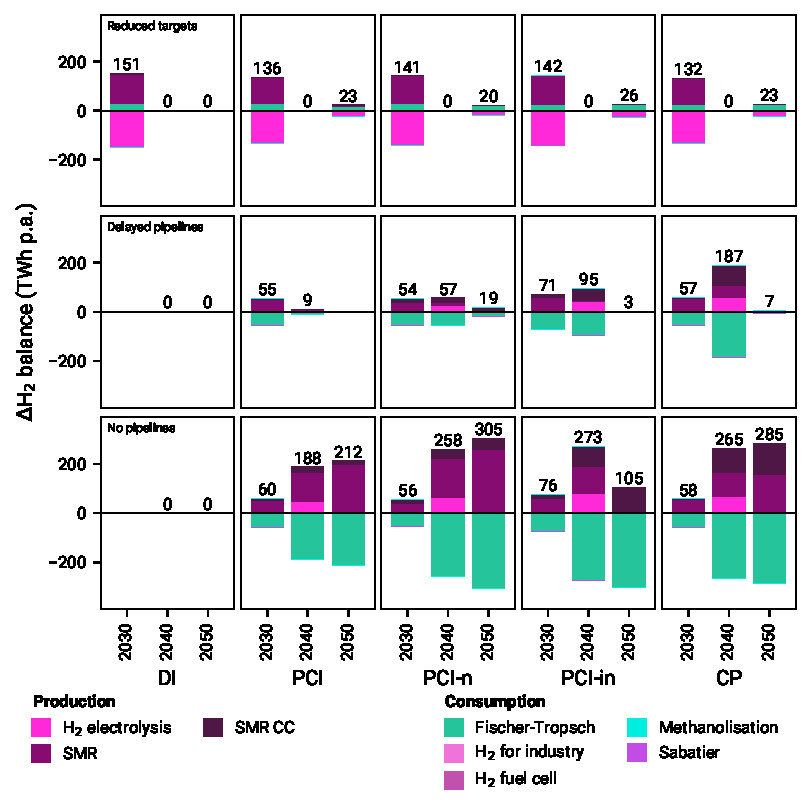
\includegraphics[width=0.49\textwidth]{balances_overview_extended_H2}
  \end{figure}
\end{frame}

\begin{frame}{\textbf{Why H$_2$?} Most H$_2$ is used for derivative fuels and chemicals!}
  
  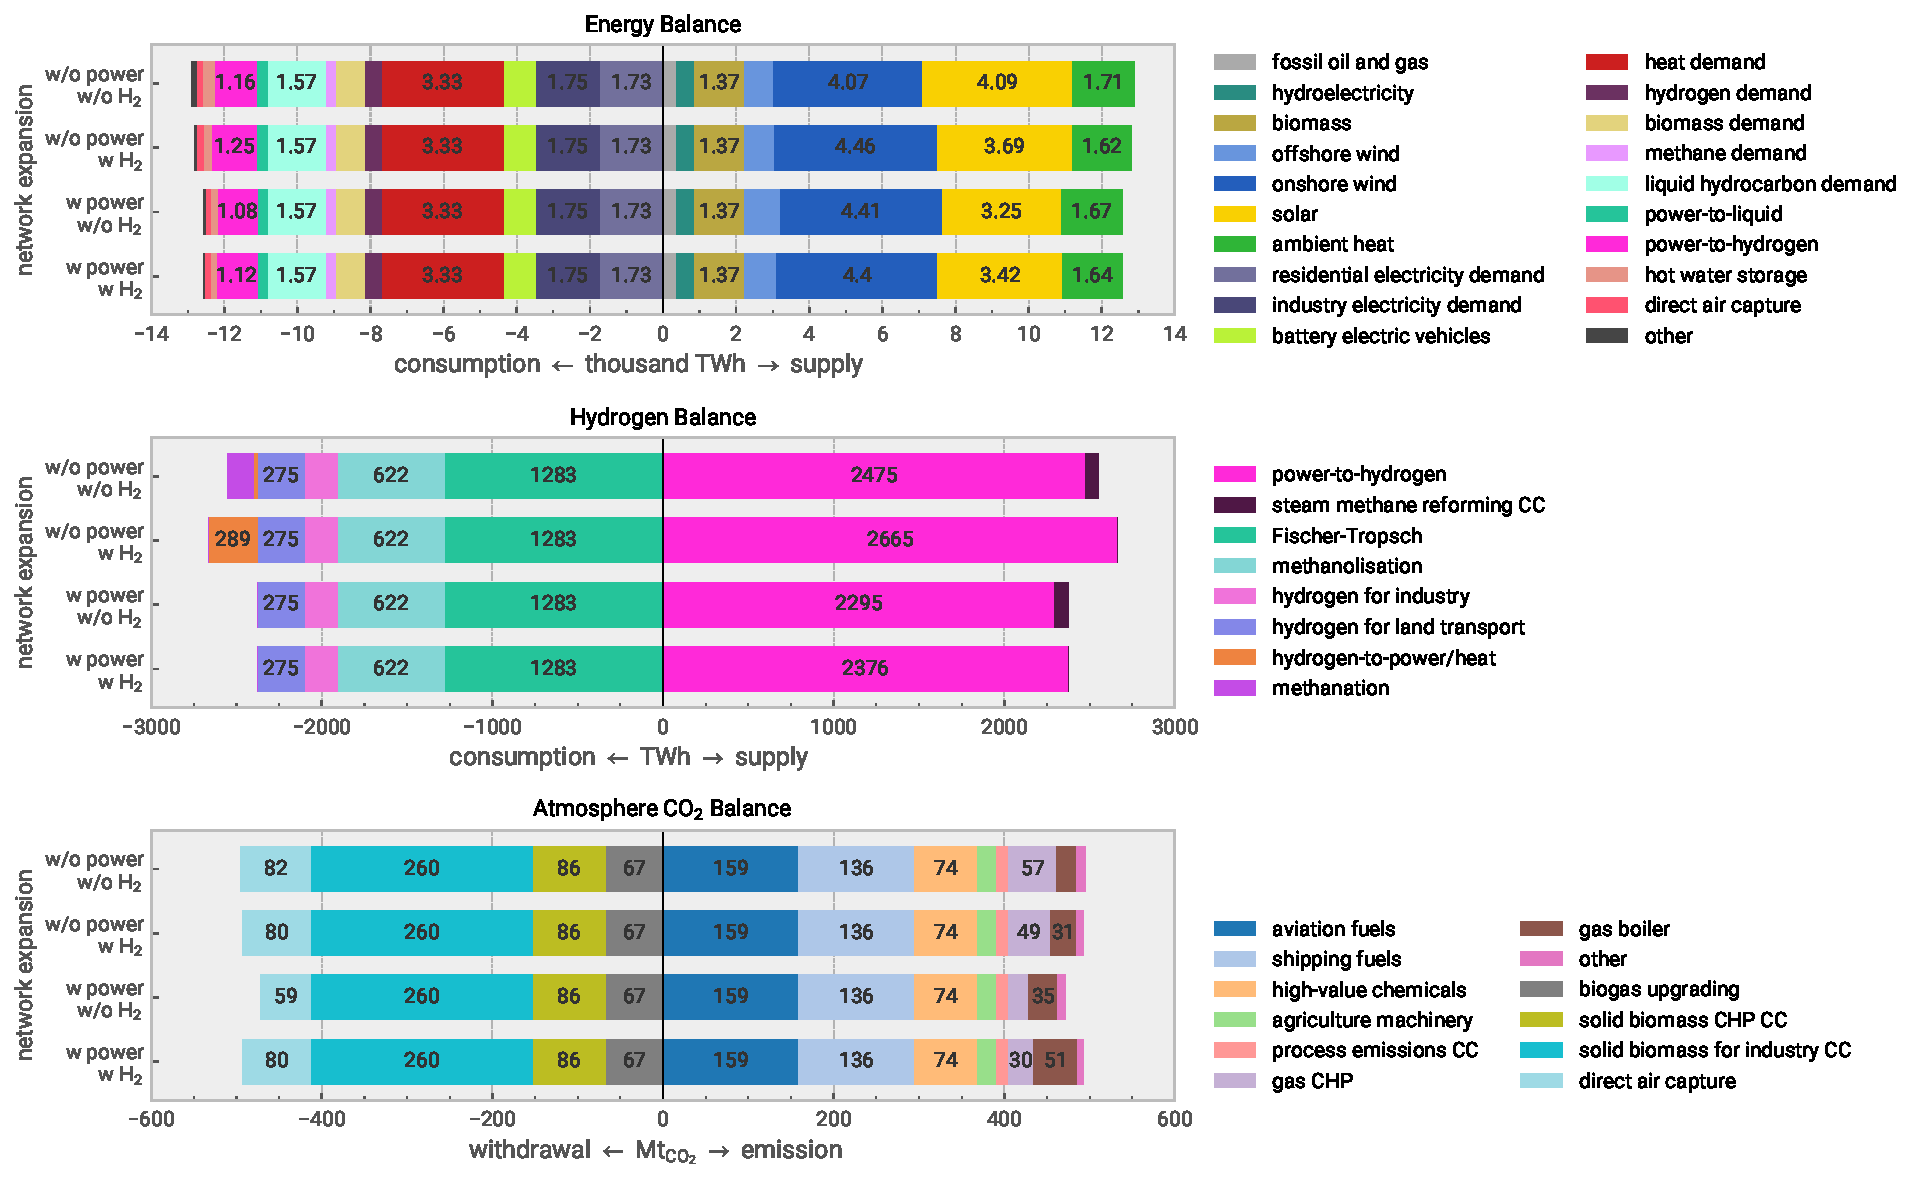
\includegraphics[width=1.2\textwidth, trim=0cm 6.6cm 0cm 6.6cm, clip]{other/hydrogen_balance.pdf}

  \footnotesize

  Mostly \alert{green electrolytic hydrogen supply}. \alert{Few direct uses of hydrogen} in the energy system, but it is
  used to synthesise other fuels and chemicals:

  \begin{multicols}{2}
  \begin{itemize}
    \item ammonia for fertilizers
    \item direct reduced iron for steelmaking
    \item shipping and aviation fuels
    \item precursor to high-value chemicals
    \item backup heat and power supply
    \item some heavy duty land transport
  \end{itemize}
  \end{multicols}

  \source{Neumann, Zeyen, Victoria, Brown, 2023\\\url{https://doi.org/10.1016/j.joule.2023.06.016}}
\end{frame}

\begin{frame}{Transporting \textbf{CO$_2$ to H$_2$} or transporting \textbf{H$_2$ to CO$_2$}?}
  
  \centering
  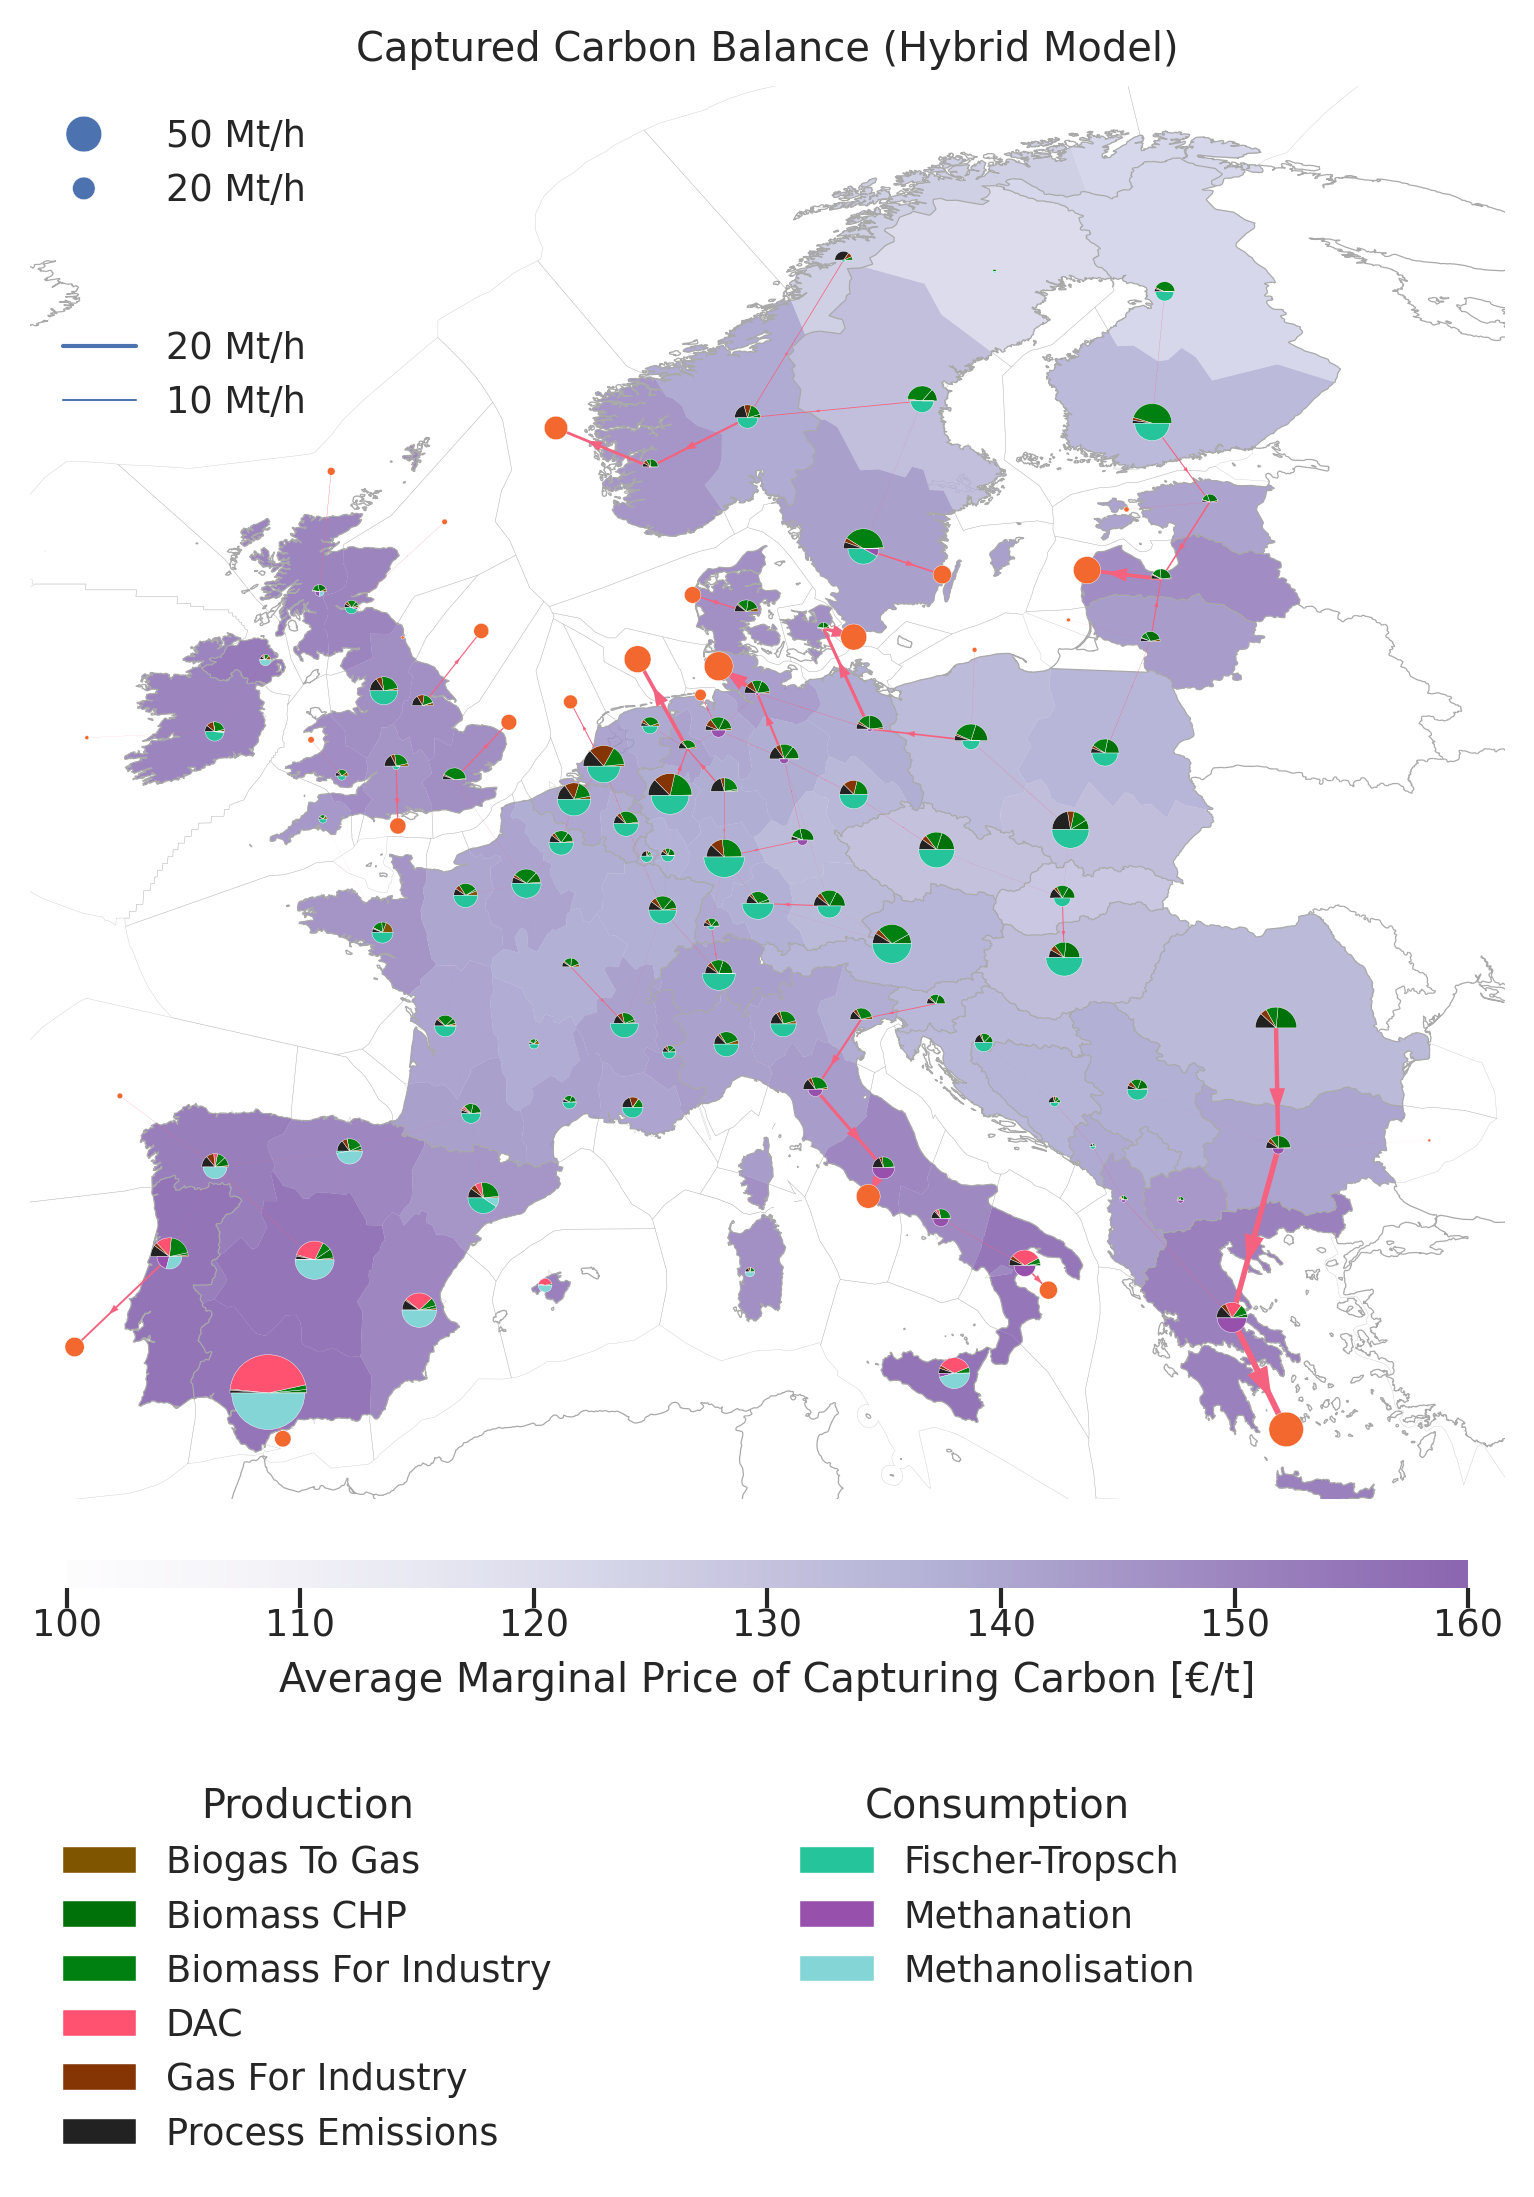
\includegraphics[width=0.35\textwidth]{other/carbon_networks_balance_map_carbon}
  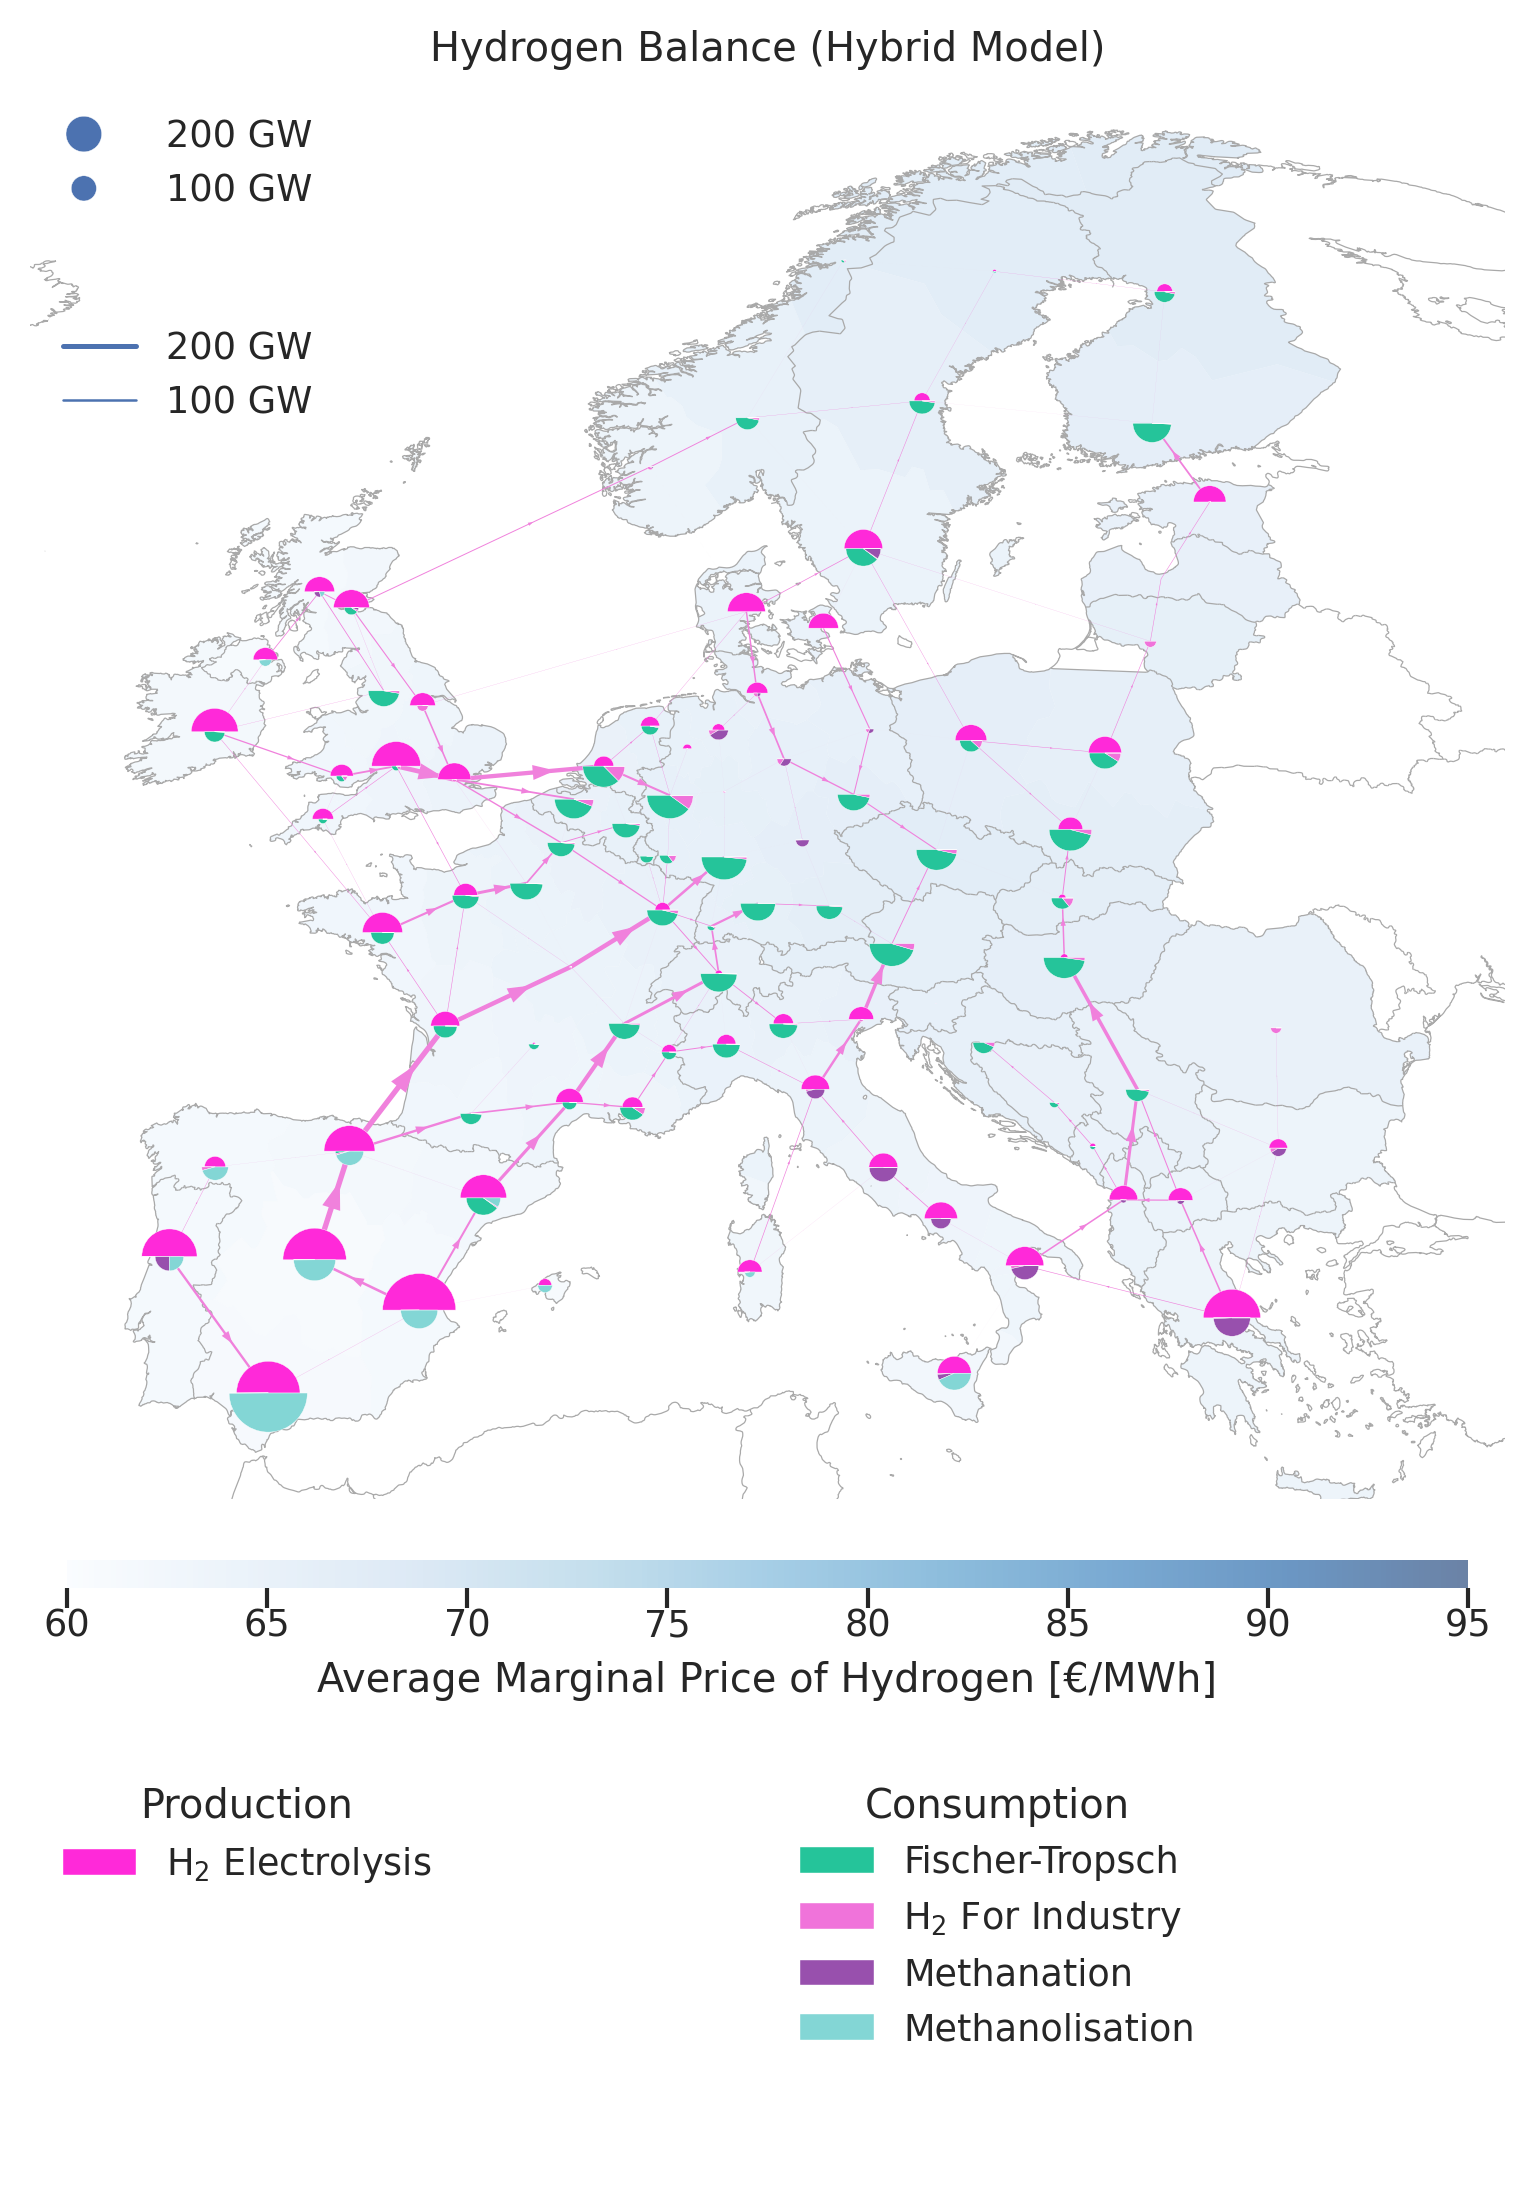
\includegraphics[width=0.35\textwidth]{other/carbon_networks_balance_map_hydrogen}

  \source{Hofmann, Tries, Neumann, Zeyen, Brown, 2024\\\url{https://arxiv.org/abs/2402.19042}}

\end{frame}


\begin{frame}{\textbf{Carbon management}: Capture, use, transport and sequestration}
  
  \begin{center}
    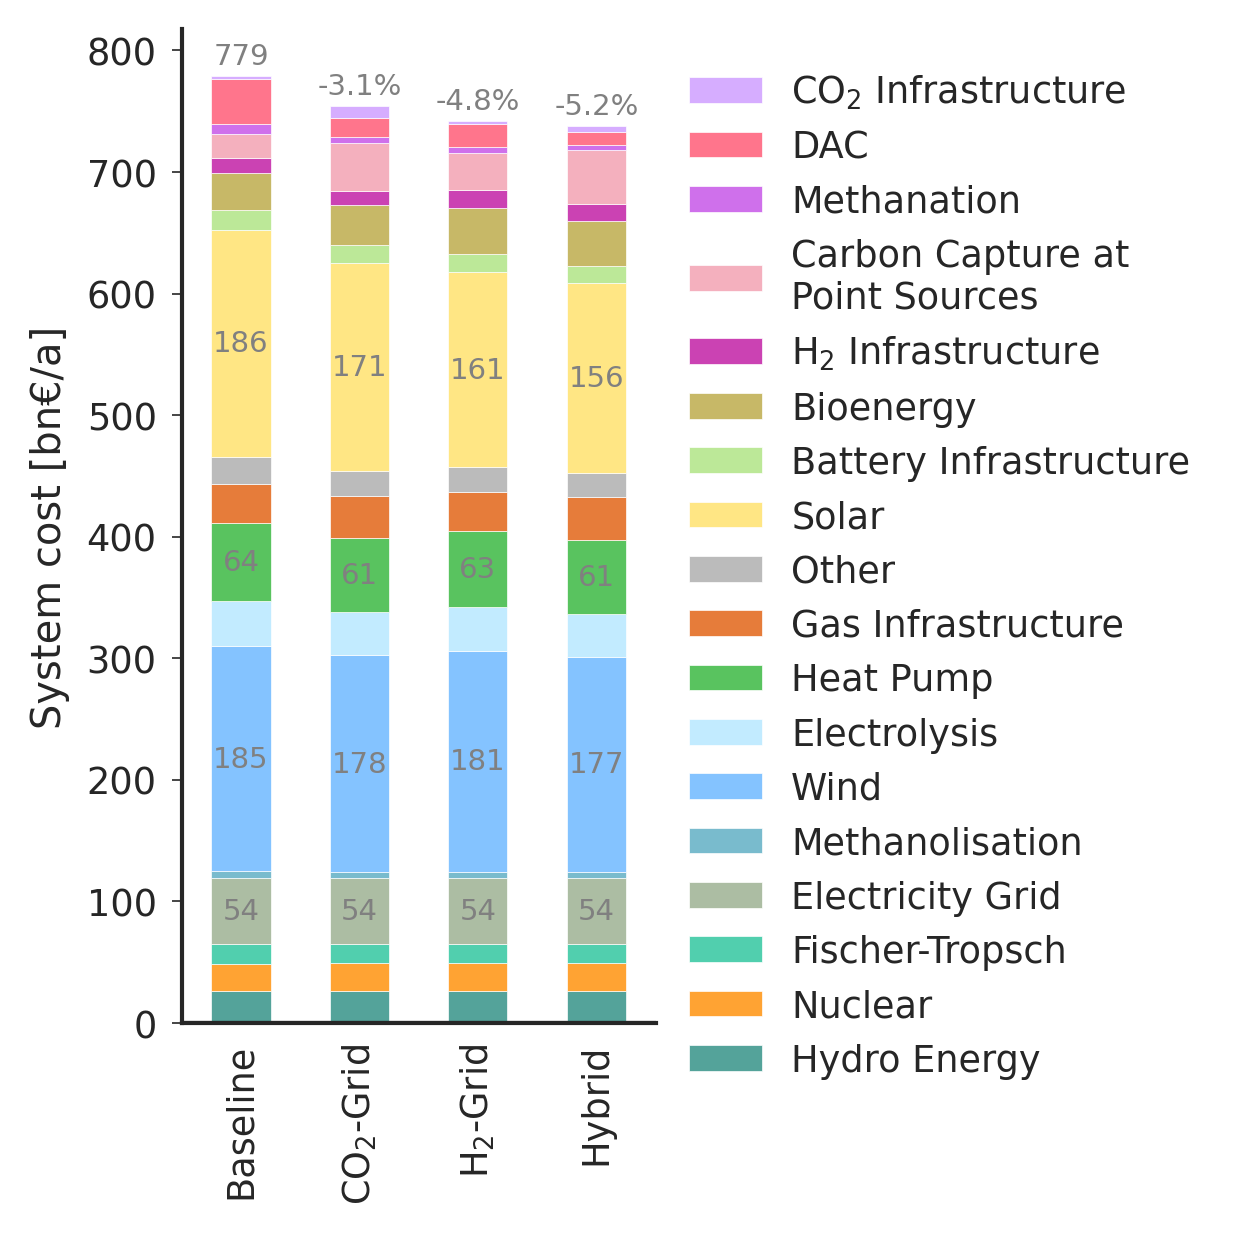
\includegraphics[height=0.73\textheight]{other/carbon_networks_cost_bar}
    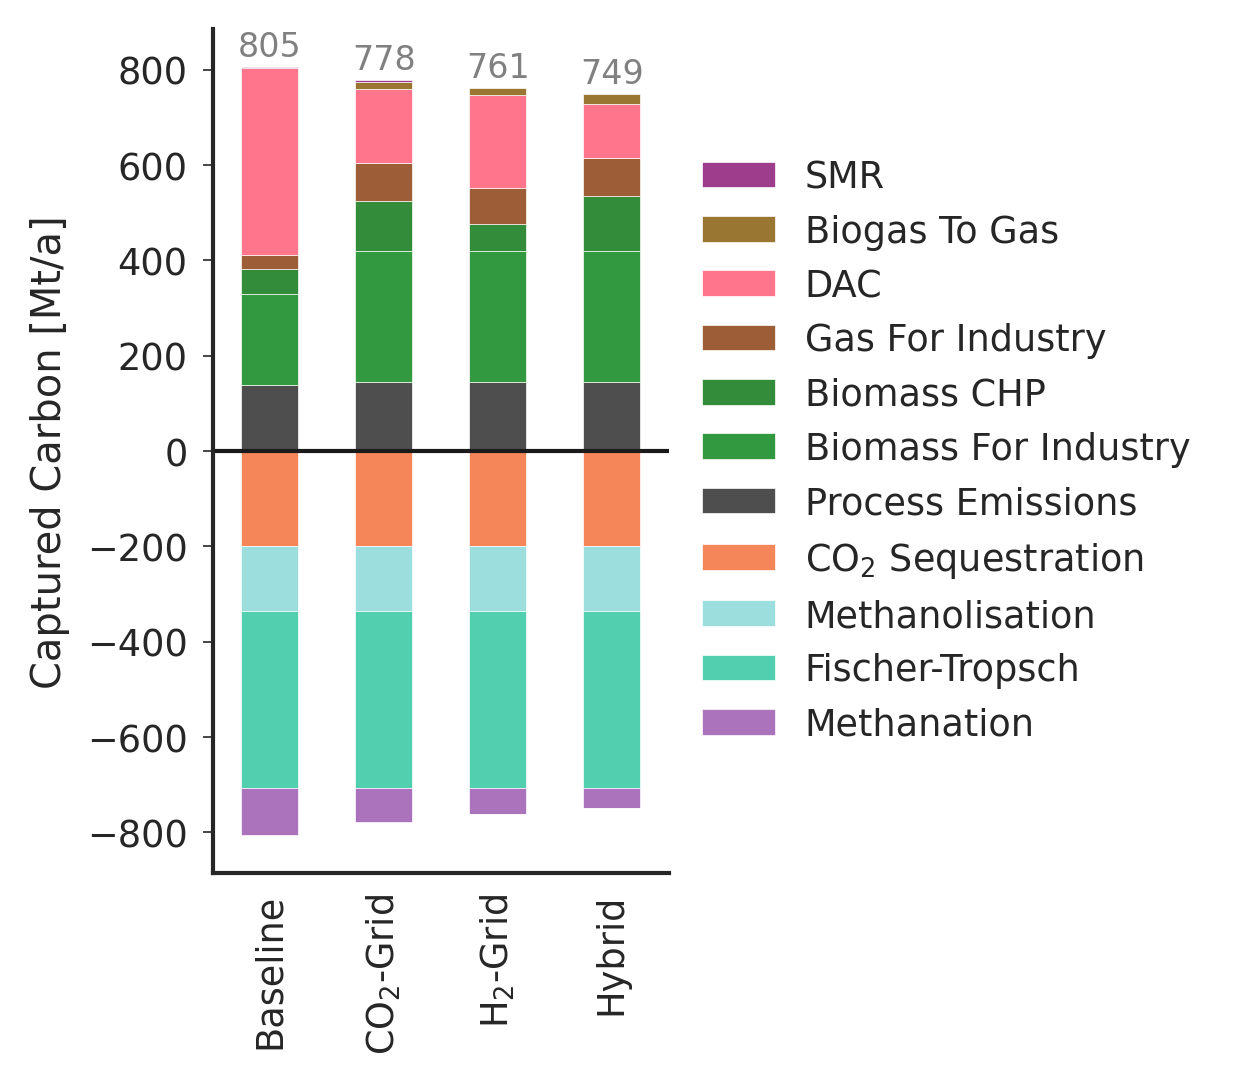
\includegraphics[height=0.71\textheight]{other/carbon_networks_balance_bar_carbon}

    \vspace{-0.25cm}
    \footnotesize
    \begin{itemize}
      \item \alert{CCS} for process emissions (for instance, in cement industry)
      \item \alert{CCU} for e-synfuels and e-chemicals (in particular, shipping, aviation, plastics)
      \item \alert{CDR} for unabatable and negative emissions (to offset imperfect capture rates)
    \end{itemize}

  \end{center}

  \source{Hofmann, Tries, Neumann, Zeyen, Brown, 2024\\\url{https://arxiv.org/abs/2402.19042}}

\end{frame}

\begin{frame}{Electricity high-voltage grid based on OpenStreetMap (OSM)}

  \begin{columns}
    \begin{column}{0.64\textwidth}
      \footnotesize
      \begin{itemize}
        \setlength\itemsep{.8em}
        \item Dataset contains a topologically connected representation of the European high-voltage grid (220 kV to 750 kV) constructed using OpenStreetMap data
        \item Heuristic cleaning process was used to for lines and links where electrical parameters are incomplete, missing, or ambiguous
        \item Close substations within a radius of 500 m are aggregated to single buses
        \item Unique transformers are added for each voltage pair in a substation
        \item AC lines mapped using pandapower's standard line type library. In default version, nominal capacity is set to 70 \% of the technical capacity to account for n-1 security approximation
        \item Includes all 38 European HVDC connections with their nominal rating that are commissioned as of 2024
      \end{itemize}
    \end{column}
    \begin{column}{0.36\textwidth}
      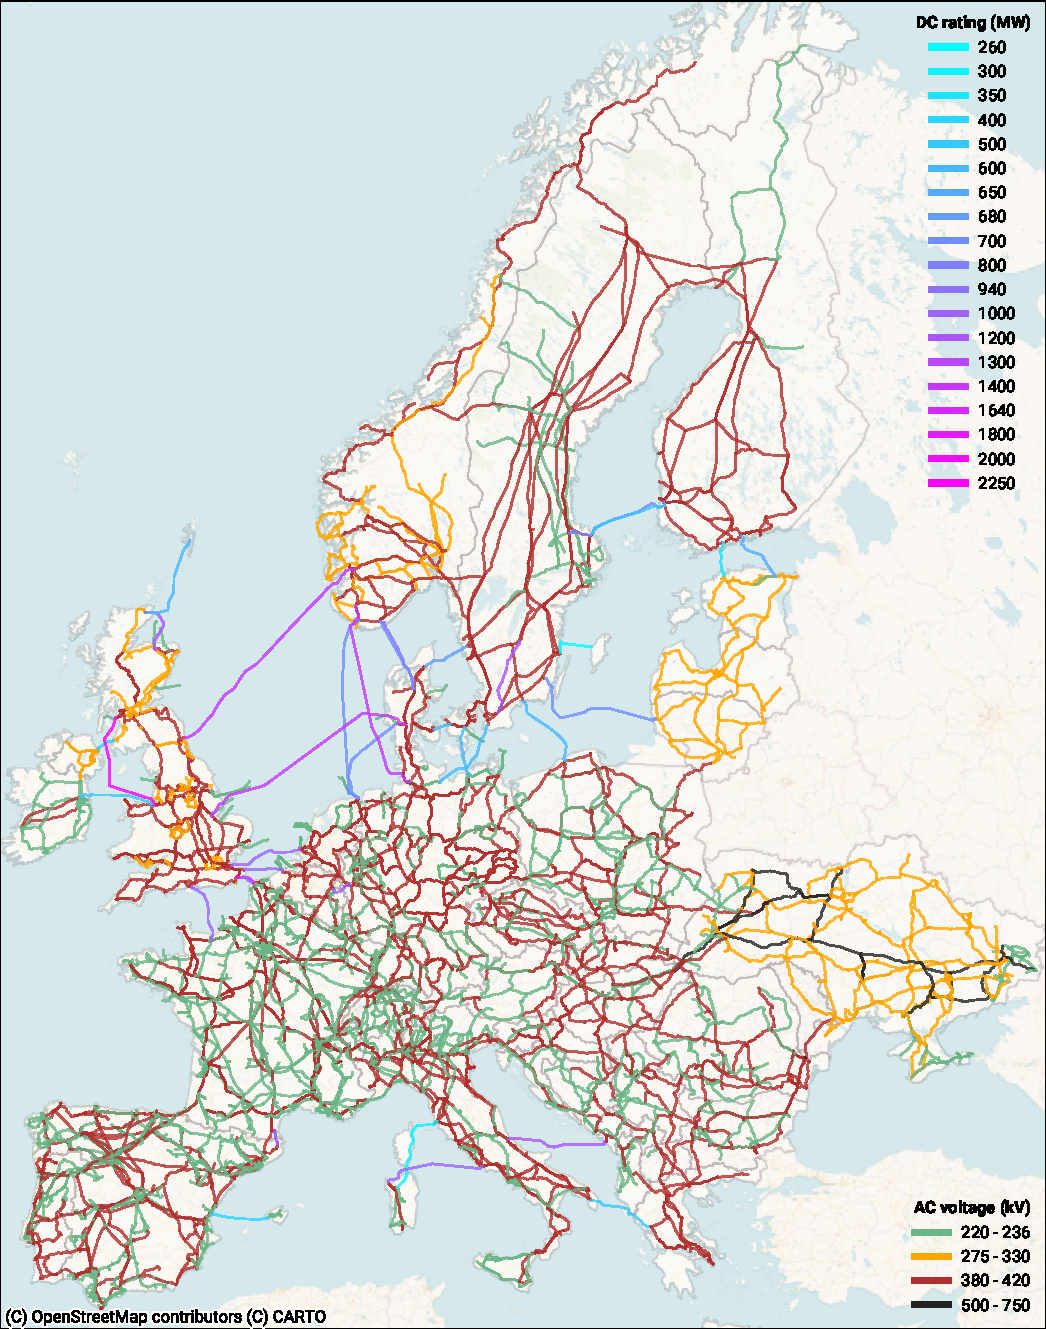
\includegraphics[width=1\textwidth]{osm_map}
    \end{column}
  \end{columns}
  \source{Own illustration based on data extracted using Overpass Turbo API\\\url{https://openstreetmap.org}}
  
  
\end{frame}

\end{document}